\documentclass[12pt]{article}
\usepackage{amssymb}
\usepackage{geometry}
\usepackage{amsmath, amsfonts, bm, graphicx}
\usepackage{float,mathrsfs}
\usepackage{multicol}

\geometry{margin=1in}
\title{}
\date{}
\author{}
\newcommand{\vol}{\mathord{\text{\ooalign{\hidewidth $V$\hidewidth\cr\kern-0.5pt\raisebox{0.8ex}{\rule[0pt]{1em}{0.5pt}}}}}}
\begin{document}

\begin{center}
{\LARGE ESC-251 Systems Engineering\par}
\end{center}
\section*{Systems}
A system is a combination of interacting components that produces an output in response to an input. Systems can be mechanical, electrical, chemical, etc. The behavior of a system can be described using mathematical models, such as differential equations or transfer functions.
\begin{center}
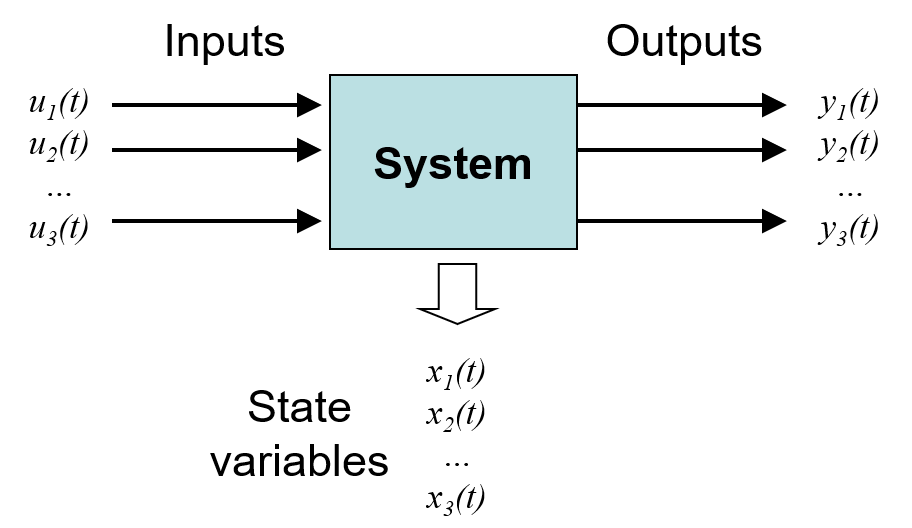
\includegraphics[width=0.5\textwidth]{Systems.png}
\end{center}
\textbf{Static Systems}\\
Output depends only on the current input and does not change with time, once the input stops, the output stops (ie. static displacement of a spring).\\\\
\textbf{Dynamic Systems}\\
Output depends on past and current inputs, and changes over time (ie. driven oscillators).\\\\
\textbf{Parameter Variation}
\begin{itemize}
    \item \textbf{Time-varying}: coefficients of the system change with time (ie. changing mass or spring stiffness).
    \item \textbf{Time-invariant}: coefficients of the system do not change with time (ie. constant mass and spring stiffness).
\end{itemize}
For this course, we will focus on linear, time-invariant (LTI) systems. This means that the system's \textit{equations of motion} are linear, and the coefficients do not change with time. A property of time-invariant systems is that a time delay in the input only delays the output by the same amount, with no dependence on the absolute time.\\\\
Linear systems also obey \textbf{superposition}, which means that its response to multiple inputs is the sum of its responses to each input \textit{individually}.\\\\
Generally, our approach to systems analysis will be to model elements mathematically to derive the equations of motion. Then, we use the Laplace transform to the differential equations to either find the \textbf{transfer function} (the ratio of the output to the input in the Laplace domain $s$) or the response of the system in the time domain (solution of the differential equation).
\newpage
\begin{center}
{\LARGE Math Review\par}
\end{center}
\section*{Complex Numbers}
In systems we use $j=\sqrt{-1}$ instead of $i$ to avoid confusion with current.\\\\
\textbf{Complex Vector Representation}\\
\begin{minipage}{0.5\textwidth}
Rectangular form:
\[\vec{X} = a + jb\]
Polar form:
\[\vec{X} = M\angle \phi\]
Complex Exponential form:
\[\vec{X} = Me^{j\phi}\]
Where:
\[\boxed{M = \sqrt{a^2 + b^2}, \quad \phi = \arctan\left(\frac{b}{a}\right)}\]
\[\implies a = M\cos(\phi), \quad b = M\sin(\phi)\]
\end{minipage}
\hfill
\begin{minipage}{0.5\textwidth}
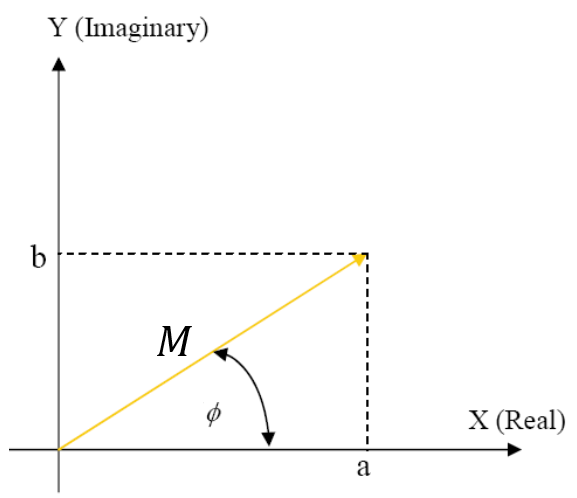
\includegraphics[width=\textwidth]{Complex Vector.png}
\end{minipage}\\\\
\underline{Note:} $arctan$ has a range of $(-\pi/2, \pi/2)$, so we have to add or subtract $\pi$ to get the correct angle based on the quadrant of the complex number.\\\\
\textbf{Euler's Identity}
\[\boxed{e^{j\phi} = \cos(\phi) + j\sin(\phi)}\]
\textbf{Complex Conjugate}\\
The complex conjugate of $\vec{X} = a + jb$ is $\vec{X}^* = a - jb$. In polar form, the complex conjugate is $M\angle -\phi$.\\\\
\textbf{Operations}\\
Addition/Subtraction:
\[(a+jb) + (c+jd) = (a+c) + j(b+d)\]
Multiplication/Division:
\[(a+jb)(c+jd) = (ac - bd) + j(ad + bc)\]
\[\frac{a+jb}{c+jd} = \frac{(a+jb)(c-jd)}{(c+jd)(c-jd)} = \frac{(ac + bd) + j(bc - ad)}{c^2 + d^2}\]
\underline{Using Complex Exponential Form:}\\
Multiplication:
\[\left(M_1 e^{j\phi_1}\right) \left(M_2 e^{j\phi_2}\right) = M_1 M_2 e^{j(\phi_1 + \phi_2)}\]
Division:
\[\frac{M_1 e^{j\phi_1}}{M_2 e^{j\phi_2}} = \frac{M_1}{M_2} e^{j(\phi_1 - \phi_2)}\]
\underline{Note:} Multiplying by $j$ is equal to \textit{adding} a phase shift of $90^\circ$ (or $\pi/2$ radians) in the complex plane.
\[j = e^{j\frac{\pi}{2}}\]
Also, if $z$ and $w$ are complex numbers, then:
\[|zw| = |z||w|\]
But
\[|z + w| \neq |z| + |w|\]
\section*{Differential Equations}
\textbf{Linear First Order Differential Equation}\\
For a first-order linear differential equation of the form:
\[\frac{dy}{dx} + p(t)y = g(t)\]
Method:\\
Find the integrating factor:
\[\boxed{\mu(t) = e^{\int p(t) dt}}\]
The solution is given by:
\[\boxed{y(t) = \frac{1}{\mu(t)}\int \mu(t)g(t) dt}\]
\textbf{Linear Second Order Differential Equation}\\
For higher order homogeneous linear differential equations with constant coefficients of the form, we can use the characteristic equation to find the \textit{homogeneous solution} (right hand side equals zero).\\\\
Method:\\
Given a homogeneous linear differential equation with constant coefficients:
\[ay'' + by' + cy = 0\]
We assume the solution of the form:
\vspace{-1em}
\begin{eqnarray*}
y(t) &=& e^{rt}\\
y'(t) &=& re^{rt}\\
y''(t) &=& r^{2}e^{rt}\\
\end{eqnarray*}
Then,  
\vspace{-1em}
\[ar^{2}+br+c=0\]
We can solve for the roots $r$ using the quadratic formula:
\[r=\frac{-b\pm\sqrt{b^2-4ac}}{2a}\]
\underline{Note:} For higher order differential equations, we would get a polynomial of degree $n$, and we would solve for the roots by factoring.\\\\
\underline{Case 1: Real and Unique Roots}\\
For roots $r_1$ and $r_2$, the general solution is:
\[\boxed{y(t) = c_1 e^{r_1 t} + c_2 e^{r_2 t}}\]
\underline{Case 2: Complex Roots}\\
For roots $\alpha \pm \beta j$, the general solution is:
\[\boxed{y(t) =   c_1 e^{\alpha t}\cos \beta t + c_2 e^{\alpha t} \sin \beta t}\]
\underline{Case 3: Repeated Roots}\\
For repeated root $r$, the general solution is:
\[\boxed{y(t) = c_1 e^{r t} + c_2 t e^{r t}}\]
Finally, we solve for the \textbf{particular solution} (non-zero input/forcing function) using the method of undetermined coefficients. We guess the form of the particular solution and solve for the coefficients by plugging it into the differential equation.\\\\
The \textbf{general solution} is the sum of the homogeneous and particular solutions:
\[\boxed{y(t) = y_h(t) + y_p(t)}\]
\section*{Laplace Transform}
Laplace transform is the method we will mainly use to solve the differential equations of systems. It requires us to know the initial conditions of the system, but transfer functions (discussed later) assume \textit{zero initial conditions}.\\\\
Method:\\
To solve a differential equation with given initial conditions using Laplace transforms:
\begin{enumerate}  
    \item Apply the Laplace transform $\mathscr{L}$ to both sides of the differential equation. This transforms the differential equation to an algebraic equation in the $s$-domain in terms of $Y(s)=\mathscr{L}\{y(t)\}$.
    
    \item Solve the algebraic equation for $Y(s)$.
    
    \item Apply the inverse Laplace transform $\mathscr{L}^{-1}$ to find $y(t)$, converting from the $s$-domain back to the time domain.
\end{enumerate}
Typically, partial fraction decomposition is needed to find the inverse Laplace transform.
\newpage\noindent
\textbf{Laplace Transform Formulas (From Diff Eq. Notes)}
\begin{center}
\renewcommand{\arraystretch}{2}
\[
\begin{tabular}{|p{5cm}||p{5cm}|}
\hline
$f(t)$ & $F(s)$ \\
\hline\hline
$1$ & $\dfrac{1}{s}$ \\
\hline
$t^{n}$ & $\dfrac{n!}{s^{n+1}}$ \\
\hline
$e^{at}$ & $\dfrac{1}{s-a}$ \\
\hline
$\sin(at)$ & $\dfrac{a}{s^{2}+a^{2}}$ \\
\hline
$\cos(at)$ & $\dfrac{s}{s^{2}+a^{2}}$ \\
\hline
$\sinh(at)$ & $\dfrac{a}{s^{2}-a^{2}}$ \\
\hline
$\cosh(at)$ & $\dfrac{s}{s^{2}-a^{2}}$ \\
\hline
$\mathscr{U}(t-a)$ & $\dfrac{e^{-as}}{s}$ \\
\hline
$\mathscr{U}(t-a)f(t-a)$ & $e^{-as}F(s)$ \\
\hline
$e^{at}f(t)$ & $F(s-a)$ \\
\hline
$t^n f(t)$ & $(-1)^n\dfrac{d^n}{ds^n}F(s)$ \\
\hline
$\sin(at)-at\cos(at)$ & $\dfrac{2a^3}{(s^2+a^2)^2}$ \\
\hline
$t\sin(at)$ & $\dfrac{2as}{(s^2+a^2)^2}$ \\
\hline
$f * g$ & $F(s)G(s)$ \\
\hline
$\delta(t-a)$ & $e^{-sa}$ \\
\hline
$f'(t)$ & $sF(s)-f(0)$ \\
\hline
$f''(t)$ & $s^2F(s)-sf(0)-f'(0)$ \\
\hline
\end{tabular}
\]
\end{center}

\section*{Cover-Up/Limit Method}
For solving partial fraction decomposition to find the inverse Laplace transform, we can use the cover-up/limit method to find the coefficients of the factors in the denominator. 
\begin{itemize}
    \item \underline{\textbf{Distinct Linear Factors:}}
    \[ \frac{P(x)}{(x-a)(x-b)(x-c)} = \frac{A}{x-a} + \frac{B}{x-b} + \frac{C}{x-c} \]
    
    To find the coefficients, we use:
    \[A = \lim_{x \to a} \left[ (x-a) \frac{P(x)}{(x-a)(x-b)(x-c)} \right]\]
    \begin{itemize}
        \item ``Cover up'' factor in denominator
        \item Evaluate at the ``root''
    \end{itemize}

    \item \textbf{Ex:}
    \[ \frac{5x+3}{(x-1)(x-2)} = \frac{A}{x-1} + \frac{B}{x-2} \]
    \begin{itemize}
        \item[] $A = \frac{5x+3}{x-2} \Big|_{x=1} = -8$
        \item[] $B = \frac{5x+3}{x-1} \Big|_{x=2} = 13$
    \end{itemize}
\end{itemize}

\begin{itemize}
    \item \underline{\textbf{Repeated Linear Factors (Derivative Limit Method):}}
    \[ F(x) = \frac{P(x)}{G(x)(x-a)^n} = \underbrace{\frac{A_1}{x-a} + \frac{A_2}{(x-a)^2} + \dots + \frac{A_n}{(x-a)^n}}_{\text{factors of } (x-a)^n} + \dots \text{(terms for the factors of } G(x) ) \]

    For the $k^{th}$ coefficient:
    \[ A_k = \frac{1}{(n-k)!} \lim_{x \to a} \left\{ \frac{d^{n-k}}{dx^{n-k}} \left[ (x-a)^n F(x) \right]\right\} \]
    \begin{itemize}
        \item When $k=n$ (the highest order factor), we have the same formula as for distinct linear factors.
        \item We use the derivative to ``recover'' the lower order roots.
    \end{itemize}

    \item \textbf{Ex:}
    \[ F(x) = \frac{2x+3}{(x-1)^3(x+2)} = \frac{A_1}{(x-1)} + \frac{A_2}{(x-1)^2} + \frac{A_3}{(x-1)^3} + \frac{B}{x+2} \]
    \begin{multicols}{2}
        \begin{itemize}
        \item[] $A_3 = \frac{2x+3}{x+2} \Big|_{x=1} = \frac{5}{3}$
        \item[] $A_2 = \frac{d}{dx} \left( \frac{2x+3}{x+2} \right) \Big|_{x=1} = \frac{1}{9}$
        \item[] $A_1 = \frac{1}{2!} \frac{d^2}{dx^2} \left( \frac{2x+3}{x+2} \right) \Big|_{x=1} = -\frac{1}{27}$
        \item[] $B = \frac{2x+3}{(x-1)^3} \Big|_{x=-2} = -\frac{1}{27}$
        \end{itemize}
    \end{multicols}
\end{itemize}
\noindent\underline{Note:} 
\begin{itemize}
    \item For irreducible quadratic factors, this doesn't apply (use $Cx+D$ and solve).
    \item Always check that $(\deg \text{ of num}) < (\deg \text{ of denom})$.
\end{itemize}
\vspace{1em}
\noindent\hrule
\vspace{1em}
\newpage
\begin{center}
{\LARGE Response Analysis\par}
\end{center}
\section*{Transfer Function}
Transfer functions relate input to output in the Laplace domain, \textit{assuming zero initial conditions}. It is defined as:
\[G(s) = \frac{Y(s)}{R(s)}\]
\begin{center}
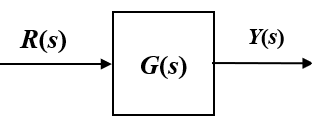
\includegraphics[width=0.3\textwidth]{Transfer Function.png}
\end{center}
Transfer functions \textit{don't capture the time domain response of the system}, because the input function is undefined. However, once we define an input function (step function, impulse, etc.), we can find the time domain response by taking the inverse Laplace transform of $Y(s) = G(s)R(s)$.\\\\
Since the transfer function assumes zero initial conditions, it captures only the \textbf{steady state response} of the system, which is the response due to the input function.\\\\
\underline{Note:} When writing out the equations of motion (time domain), write it in the form
\[\text{(output)} = \text{(input)}\]
\[\text{(dep. variables LHS)} = \text{(input RHS)}\]
\section*{Transient vs Steady State Response}
\textbf{Transient Response} is the part of the system's response that dies out over time, while \textbf{Steady State Response} is the part of the response that remains after the transient response has decayed.\\\\
Typically, the steady state response is due to an input to the system, this input can either be a forcing function (unit-impulse, unit-step, etc.) or some static (constant) input. The transient response is due to the initial conditions ($x_0$, $v_0$, etc.) of the system. Recall that the homogeneous solution corresponds to the transient response, while the particular solution corresponds to the steady state response.
\newpage
\section*{Stability}
In terms of natural (unforced/free) response,
\begin{itemize}
    \item System is \textbf{stable} if $x(t) \to 0$ as $t \to \infty$
    \item System is \textbf{unstable} if $x(t) \to \infty$ as $t \to \infty$
    \item System is \textbf{marginally stable} if natural response neither decays nor grows but remains constant or oscillates
\end{itemize}
In terms of total response,
\begin{itemize}
    \item System is \textbf{stable} if \textit{every} bounded input yields a bounded output \textbf{(BIBO)}
    \item System is \textbf{unstable} if \textit{any} bounded input yields an unbounded output
\end{itemize}
Mathematically, we can determine stability by looking at the roots of the characteristic equation which are the \textit{poles} of the transfer function (a pole is a value of $s$ that makes the denominator of the transfer function zero):
\begin{itemize}
    \item Negative Real Part ($\text{Re}[s] < 0$) $\to$ \textbf{Stable}
    \item Positive Real Part ($\text{Re}[s] > 0$) $\to$ \textbf{Unstable}, grows exponentially
    \item One zero at $s = 0$ and one negative root $\to$ \textbf{Neutrally or marginally stable} (the negative root decays to zero, but the zero root stays constant, so its steady state response is marginally stable)
    \item Zero real part, non-zero imaginary $\to$ \textbf{Oscillatory response} (neutrally or marginally stable)
\end{itemize}
\textbf{All roots must be stable for system to be considered stable!} For example, it is possible to have stable and unstable oscillatory responses since the real part determines the amplitude of the oscillation and the imaginary part determines the frequency of the oscillation.
\begin{itemize}
    \item Positive real part (Re[$s$] $> 0$), non-zero imaginary part (Im[$s$] $\neq$ 0) $\to$ \textbf{Unstable}, flutter instability
    \item Negative real part (Re[$s$] $< 0$), non-zero imaginary part (Im[$s$] $\neq$ 0) $\to$ \textbf{Stable}, damped oscillation
\end{itemize}
\begin{center}
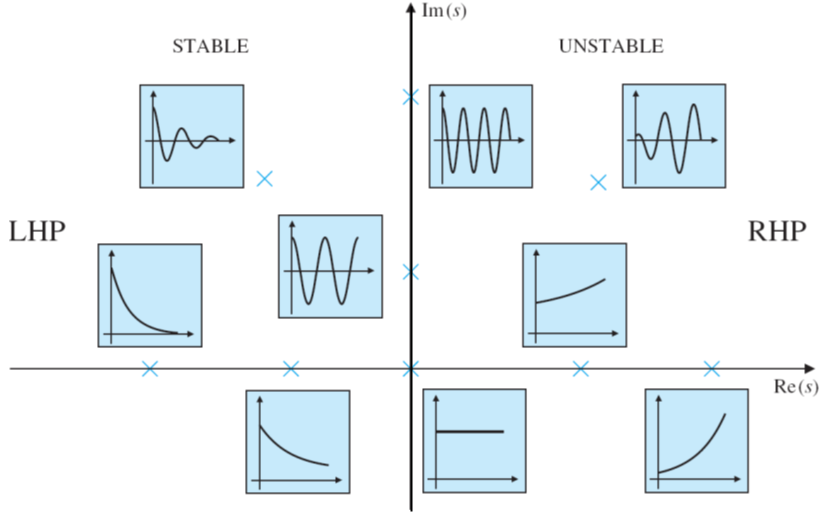
\includegraphics[width=0.7\textwidth]{Stability.png}
\end{center}
\underline{Note:} The poles of the transfer function are the values that make the denominator zero, which are the roots of the characteristic equation. The location of the poles in the complex plane determines the stability of the system.
\section*{Identifying Frequency and Time Constants}
Aside from determining the stability of a system based on its poles, we can also analyze the system's response in the time domain by looking at the time constant, natural frequency, and damping ratio of the system. These parameters can be identified from the transfer function or the characteristic equation of the system.\\\\
\textbf{Time Constant}\\
For a transfer function of a \textbf{first order system}:
\[\boxed{G(s) = \frac{K}{\tau s + 1}}\]
Where $\tau$ is the time constant and $K$ is the steady state gain.\\\\
The time constant $\tau$ describes how quickly a system reaches steady state (shorter $\tau$ means faster response). For a first order system in the time domain, the time constant is the value for $t$ such that $-Ct$ becomes $-1$:
\[v(t) = v_0 e^{-Ct}, \quad \tau = \frac{1}{C}\]
At $1\,\tau$ the system is 63.3\% of the way to its final steady state value, at $2\,\tau$ it is 86.5\%, at $3\,\tau$ it is 95\%, and at $4\,\tau$ it is 98.2\%. Thus, we can say that the system has effectively reached its steady state value after $4\,\tau$.\\\\
The steady state gain $K$ is defined as the steady state output of the system \textit{given a unit step input}. Intuitively, it describes how much the system amplifies the input at steady state.\\\\
\textbf{Natural Frequency}\\
For a \textbf{second order system with no damping}, its characteristic equation in the time and laplace domains are as follows:
\[\ddot{x} + \omega_n^2 x = 0, \quad s^2+ \omega_n^2 = 0\]
Where $\omega_n$ is the natural frequency of the system.\\\\
\textbf{Damping Ratio}\\
For \textbf{second order damped systems}, we have a non-zero damping ratio $\zeta$. For a second order system with damping, its characteristic equation is in the form:
\[\ddot{x} + 2\zeta \omega_n \dot{x} + \omega_n^2 x = 0\quad \text{or } =\frac{f(t)}{m} \quad \text{if there is a forcing function}\]
\[s^2 + 2\zeta \omega_n s + \omega_n^2 = 0 \quad \text{(in laplace domain)}\]
The damping ratio determines the nature of the system's response:
\begin{itemize}
    \item $\zeta < 0$: Unstable system (response grows exponentially).
    
    \item $\zeta = 0$: Marginally stable (undamped/free oscillations at $\omega_n$).
    
    \item $0 < \zeta < 1$: \textbf{Underdamped} (stable, oscillatory response with decaying amplitude).
    
    \item $\zeta = 1$: \textbf{Critically damped} (stable, fastest exponentially decaying return to equilibrium).
    
    \item $\zeta > 1$: \textbf{Overdamped} (stable, exponentially decaying response with slower return to equilibrium).
\end{itemize}
\underline{Note:} The \textbf{time constant of a damped second order system} is given in terms of the \textit{dominant pole} $\sigma$ (since the system has 2 poles). The dominant pole is the pole closest to the imaginary axis (the slower pole), and the time constant is given by
\[\tau = \frac{1}{\sigma}\]
The faster pole has a shorter transient response and decays to zero much faster than the slower pole and thus the dominant pole determines the overall response of the system better.
\newpage\noindent
\section*{Final/Initial Value Theorem}
We can determine the initial and final values of a system's response by just looking at the transfer function without having to find the full time domain response.\\\\
\textbf{Final Value Theorem}
\[\boxed{\lim_{t \to \infty} f(t) = \lim_{s \to 0} sF(s)}\]
\textbf{Initial Value Theorem}
\[\boxed{\lim_{t \to 0} f(t) = \lim_{s \to \infty} sF(s)}\]
\vspace{1em}
\noindent\hrule
\vspace{1em}
\newpage
\begin{center}
{\LARGE Mechanical Systems\par}
\end{center}
\section*{Distributed vs Lumped Systems}
Lumped systems are systems where the properties (mass, stiffness, damping) are concentrated at discrete points, these systems are easier to work with since we can define a finite number of degrees of freedom. Distributed systems are have properties that are distributed continuously along the system, these systems are more complex and require partial differential equations to model.
\begin{center}
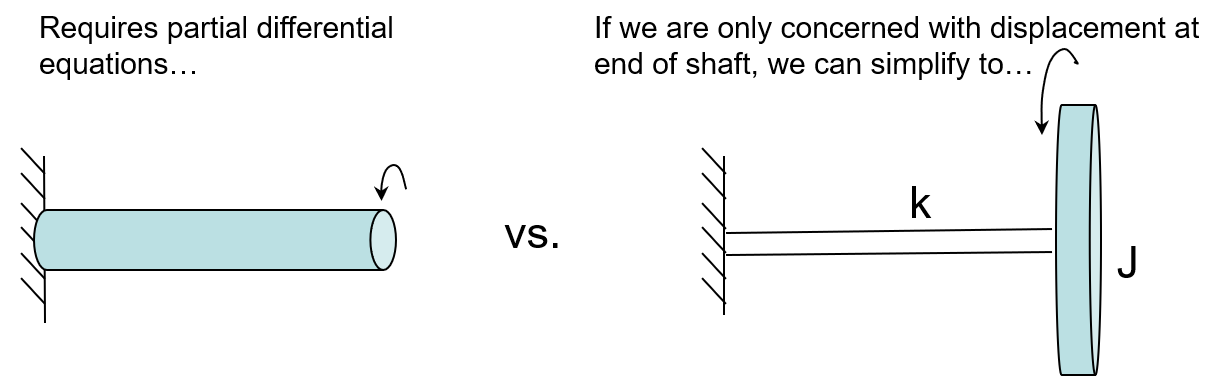
\includegraphics[width=0.7\textwidth]{Lumped.png}
\end{center}
\vspace{-2em}
\section*{Mechanical Elements}
\textbf{Inertia/Mass Elements}\\
The inertia elements of a mechanical system are the mass and moment of inertia that appear in a Newton's second law equation.
\[\sum F = ma, \quad \sum \tau = J\alpha\]
Inertia elements also store energy in the system as kinetic or potential energy. The kinetic energy of a mass is given by
\[T_{\text{trans}} = \frac{1}{2}m\dot{x}^2 \quad \text{or} \quad T_{\text{rot}} = \frac{1}{2}J\dot{\theta}^2\]
\textbf{Spring/Stiffness Elements}\\
Spring elements provide a restoring force that is proportional to the displacement of the system. The force exerted by a spring is given by Hooke's law:
\[F = kx \quad \text{or} \quad \tau = k_\text{t}\theta \quad \text{for a torsional spring}\]
and store potential energy in the system:
\[U = \frac{1}{2}kx^2 \quad \text{or} \quad U = \frac{1}{2}k_\text{t}\theta^2\]
It obeys the following assumptions:
\begin{itemize}
    \item Lumped parameter (spring is massless and has no damping)
    \item Perfectly elastic (no energy loss)
\end{itemize}
\textbf{Damping/Dissipative Elements}\\
Damping elements provide a resistive force that is proportional to the velocity of the system. The force exerted by a damper is given by:
\[F = b\dot{x}\]
It obeys the following assumptions:
\begin{itemize}
    \item No mass
    \item No energy storage (no stiffness)
    \item Is linear (force is proportional to velocity)
\end{itemize}
\section*{Power}
Power = effort $\times$ flow. In mechanical systems, effort is force and flow is velocity, so power is given by:
\[P = F \cdot v\]
In terms of rotation:
\[P = \tau \cdot \omega\]
\section*{Spring-Mass System (1 DOF)}
\begin{center}
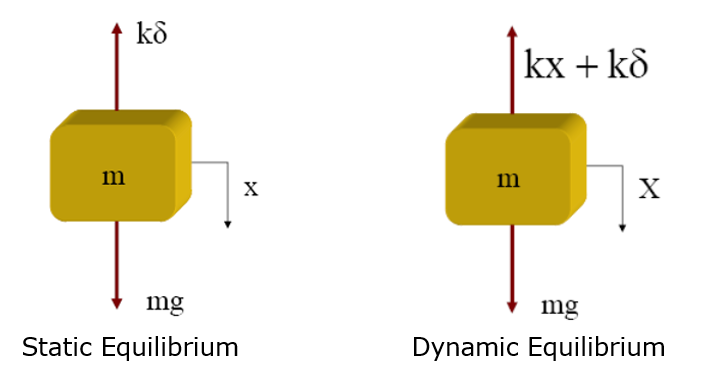
\includegraphics[width=0.7\textwidth]{Spring Mass.png}
\end{center}
An important concept for a spring–mass system is the \textit{static deflection} $\delta$, defined as the displacement of the spring under the weight of the mass. If we choose the coordinate $x$ to measure displacement from the static equilibrium position, gravity does not need to appear in the equation of motion because the weight is exactly balanced by the spring force at equilibrium, where $mg = k\delta$. The equation of motion for the system therefore becomes:
\[m\ddot{x} + kx = 0\]
\underline{Note:} We can also ignore gravitational potential energy if we choose the $x$ coordinate to measure displacement from the static equilibrium position, because the potential energy terms simplify to
\[U = \frac{1}{2}kx^2 + \text{constant}\]
However, for more complex systems, we will need to first draw the static equilibrium FBD to determine whether we can ignore gravity in the equations of motion.\\\\
\textbf{Response Due to Initial Conditions Example}\\
\begin{minipage}{0.5\textwidth}
    \begin{center}
       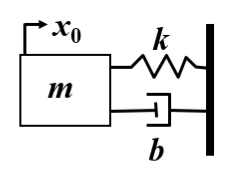
\includegraphics[width=0.5\textwidth]{Damping.png} 
    \end{center}
\[m\ddot{x}+b\dot{x}+kx = 0\]
Notice that the response reaches steady state at $x=0$ and $v=0$ because there is no forcing function, so the system is stable. The initial displacement was what generated the transient response.    
\end{minipage}
\hfill
\begin{minipage}{0.5\textwidth}
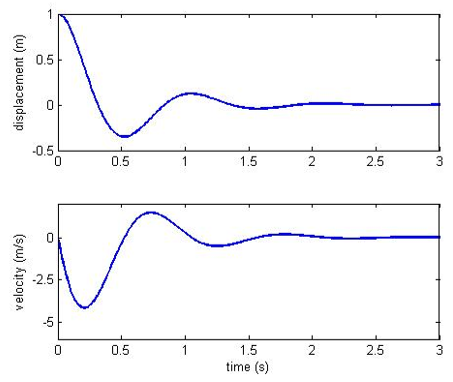
\includegraphics[width=\textwidth]{Response IC.png}
\end{minipage}
\textbf{Step Response Example}\\
\begin{minipage}{0.5\textwidth}
    \begin{center}
       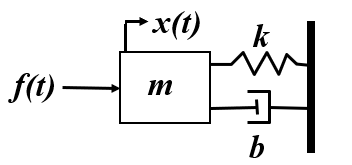
\includegraphics[width=0.5\textwidth]{Step.png} 
    \end{center}
\[m\ddot{x}+b\dot{x}+kx = f(t)\]
Notice that the response is also delayed by 1 second since the input is a step function that starts at $t=1$. Now, the steady state response is non-zero because there is a forcing function, but the transient response still decays to zero over time.
\end{minipage}
\hfill
\begin{minipage}{0.5\textwidth}
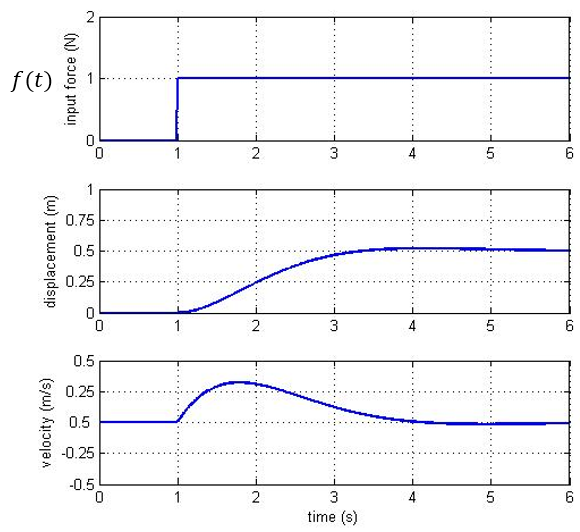
\includegraphics[width=\textwidth]{Response Step.png}
\end{minipage}
The solution via Laplace transforms is (where $1(t-1)$ is the \textbf{unit step function}):
\[
x(t)=\frac{1}{2}\cdot1(t-1)
-\frac{1}{2}e^{-(t-1)}
\left[\cos(t-1)+\sin(t-1)\right]\cdot1(t-1)
\]
\underline{Recall:} The unit step function or Heaviside function is defined as
$$ 1(t-a)=   \left\{
\begin{array}{ll}
      0 & 0\le t<a \\
      1 & t\ge a \\
\end{array}
\right.  $$
Using this function, we can represent piecewise functions as a single function. For example,
$$ f(t)=  \left\{
\begin{array}{ll}
      g(t) & 0\le t<a \\
      h(t) & t\ge a \\
\end{array}
\right.  $$
We can define this in the following way
$$f(t) = g(t)(1-1(t-a))+h(t)1(t-a)$$
We can do this using the fact that $1(t-a)$ is 0 before $t=a$ and 1 after $t=a$. Thus, $1-1(t-a)$ is 1 before $t=a$ and 0 after $t=a$.
\section*{Two DOF Systems}
A degree of freedom (DOF) is an independent coordinate that can be used to describe the configuration of a system. What makes a 2 DOF system different from a 1 DOF system is that the equations of motion are coupled, meaning that the motion of one mass affects the motion of the other mass.
\begin{center}
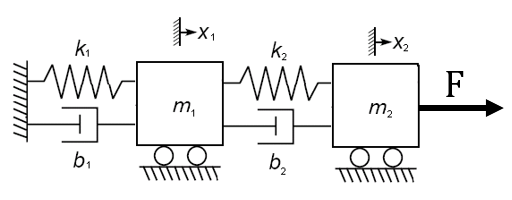
\includegraphics[width=0.6\textwidth]{2 DOF.png}
\end{center}
To solve for the equations of motion, we start with an assumption of the relative positions $x_1$ and $x_2$ of the two masses. This way we can know what direction the spring forces are acting in. Note that we are measuring $x_1$ and $x_2$ relative to their static deflections.\\\\
\underline{Assumptions:} $x_2>x_1$, $\dot{x}_2>\dot{x}_1$\\\\
Now we can draw the FBDs, keeping in mind that Newton's third law applies to the spring forces in between the two masses.
\begin{center}
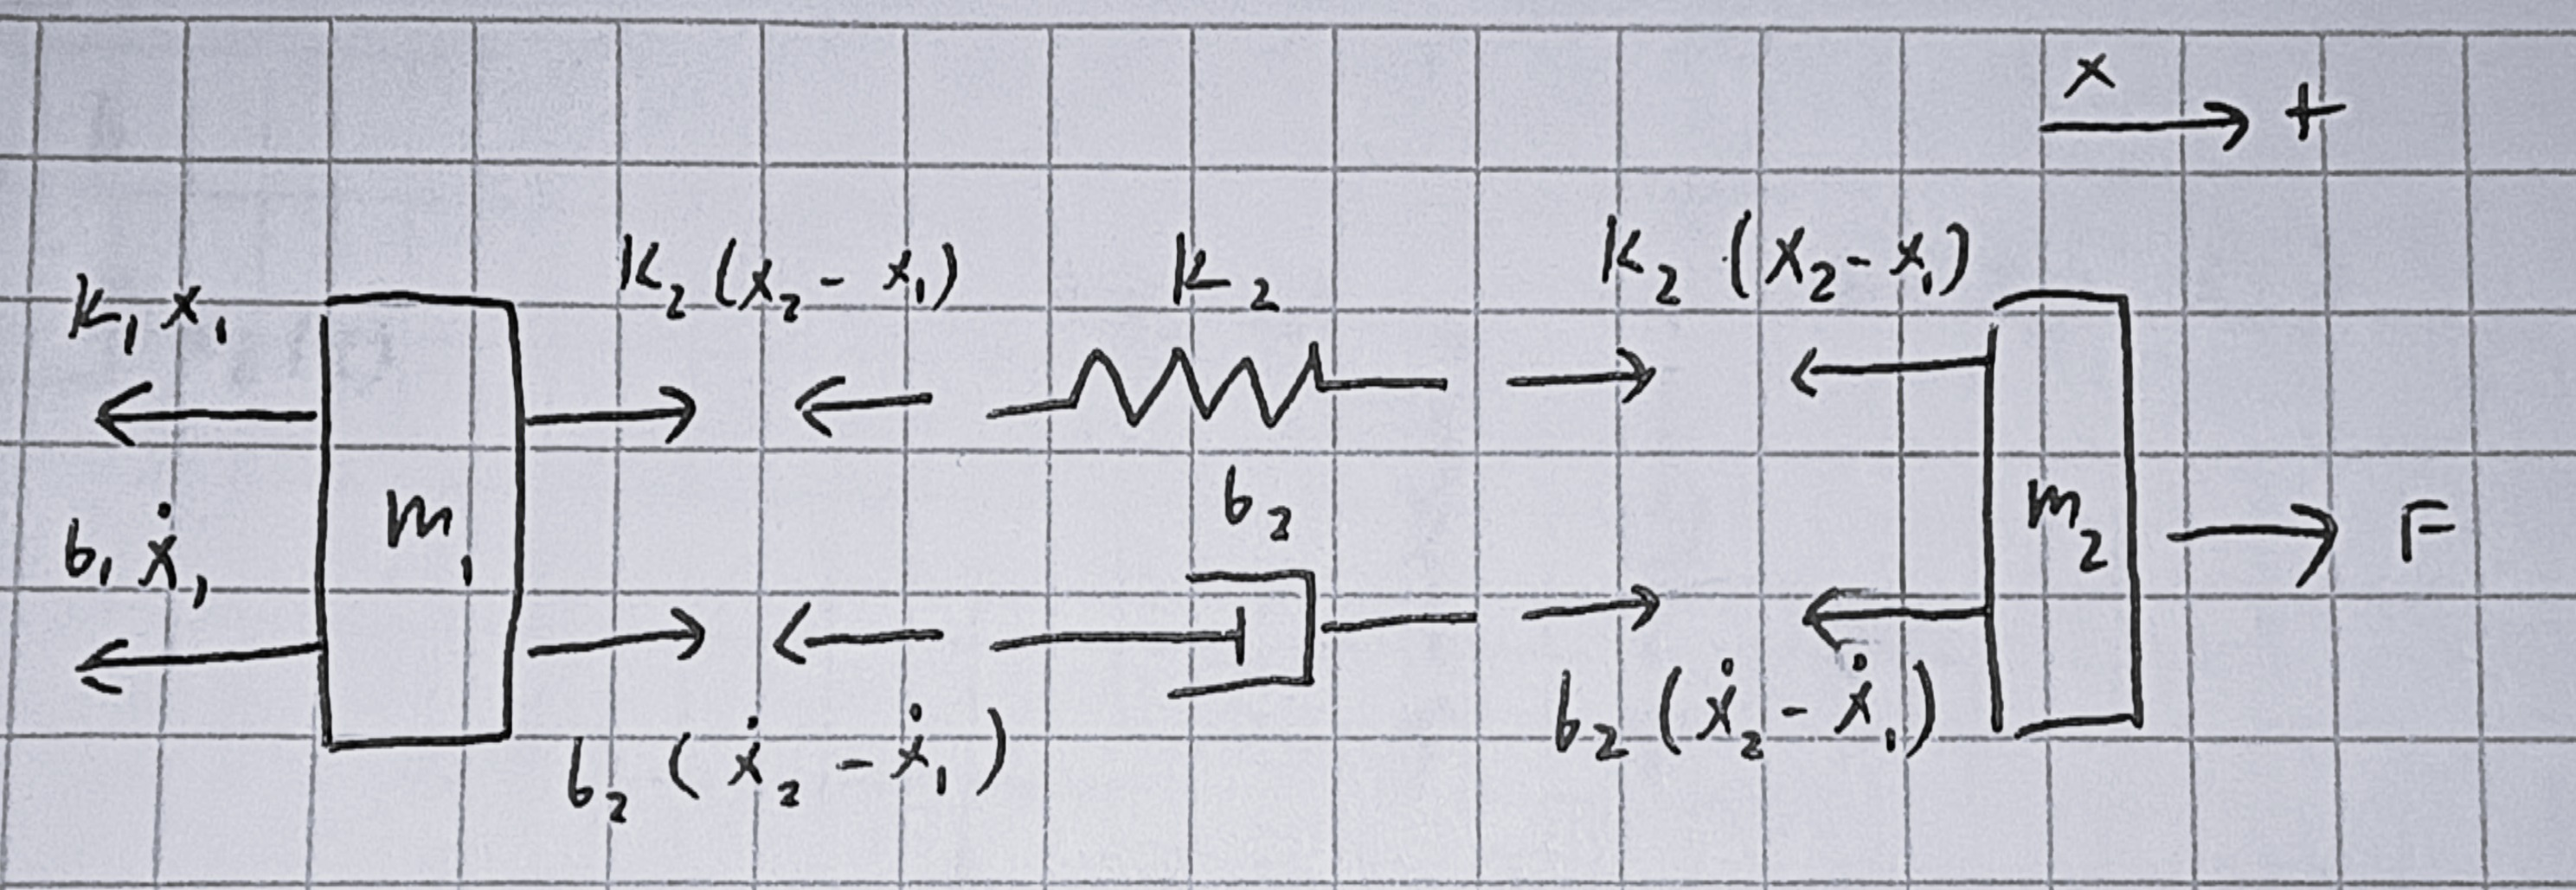
\includegraphics[width=0.7\textwidth]{FBD 2 DOF.jpg}
\end{center}
Equations of motion:
\[\sum F_1 = m_1\ddot{x}_1=-k_1x_1-b_1\dot{x}_1+k_2(x_2-x_1)+b_2(\dot{x}_2-\dot{x}_1)\]
\[\sum F_2 = m_2\ddot{x}_2=F(t)-k_2(x_2-x_1)-b_2(\dot{x}_2-\dot{x}_1)\]
Now we can apply the Laplace transform to both equations, but since they are coupled, we will have to solve the system of equations to find the transfer function for each mass (substitute one equation into the other to eliminate one of the variables).
\section*{Energy Methods}
Instead of using Newton's second law to derive the equations of motion, we can also use energy methods, which are often easier for more complex systems. The method is as follows:
\begin{itemize}
    \item Define the total kinetic energy $T$ and potential energy $U$ of the system.
    \item Because energy is conserved, we can differentiate the total energy to find the equations of motion.
    \[\boxed{\frac{d(T+U)}{dt}=0}\]
\end{itemize}
Note that this only works for conservative systems, \textit{where there is no energy loss due to damping or friction}. For non-conservative systems, it is easier to use Newton's second law to derive the equations of motion.\\\\
\textbf{Rolling Without Slipping}\\
Recall that when an object rolls without slipping, it obeys these conditions:
\begin{itemize}
    \item $v_\text{CM} = R\omega$ 
    \item $a_\text{CM} = R\alpha$
    \item $v_\text{contact} = 0$
\end{itemize}
\underline{Note:} Don't forget to include both translational and rotational kinetic energy, as well as gravitational potential energy if the system is not at static equilibrium.
\[T=\frac{1}{2}m\dot{x}^2+\frac{1}{2}J\dot{\theta}^2\]
Sometimes when using small angle approx, we will need to use higher order approximations to not have a zero after differentiating.
\section*{Combining Stiffness}
\begin{minipage}{0.5\textwidth}
    \textbf{Springs in Parallel}\\
    When two springs are in parallel, they see the \textit{same deflection} but feel different forces (if $k_1 \neq k_2$). The equivalent stiffness is the sum of the two stiffnesses:
    \[\boxed{k_\text{eq} = k_1 + k_2}\]
\end{minipage}
\hfill
\begin{minipage}{0.45\textwidth}
\begin{center}

\includegraphics[width=\textwidth]{Parallel.png}
\end{center}
\end{minipage}\\\\
\begin{minipage}{0.5\textwidth}
    \textbf{Springs in Series}\\
    When two springs are in series, they see the \textit{same force} but feel different deflections (if $k_1 \neq k_2$). The equivalent stiffness is the reciprocal of the sum of the reciprocals of the two stiffnesses:
    \[\boxed{\frac{1}{k_\text{eq}} = \frac{1}{k_1} + \frac{1}{k_2}}\]
\end{minipage}
\hfill
\begin{minipage}{0.35\textwidth}
\begin{center}

\includegraphics[width=\textwidth]{Series.png}
\end{center}
\end{minipage}\\
\textbf{Stiffness Equivalent: Buoyancy}\\
Since the buoyant force is given as:
\[\boxed{F_\text{b}=\rho g A x}\]
Where $x$ is the depth of the object in the fluid, $A$ is the cross-sectional area of the object, and $\rho$ is the density of the fluid, we can treat the buoyant force as a spring force with an equivalent stiffness of:
\[\boxed{k_\text{eq} = \rho g A}\]
\section*{Common Moments of Inertia}
\begin{itemize}
\item \textbf{Point mass} (mass $m$ at distance $r$ from axis of rotation)
\[I = mr^2\]

\item \textbf{Thin rod} (length $L$, mass $m$)
\[
I = \frac{1}{12} mL^2 
\quad \text{(about center, axis perpendicular to rod)}
\]
\[
I = \frac{1}{3} mL^2 
\quad \text{(about one end, axis perpendicular to rod)}
\]

\item \textbf{Solid disk} (radius $R$, mass $m$)
\[
I = \frac{1}{2} mR^2 
\quad \text{(about center, axis perpendicular to plane)}
\]

\item \textbf{Thin hoop / ring} (radius $R$, mass $m$)
\[
I = mR^2 
\quad \text{(about center, axis perpendicular to plane)}
\]

\item \textbf{Solid cylinder} (radius $R$, mass $m$)
\[
I = \frac{1}{2} mR^2 
\quad \text{(about central symmetry axis)}
\]

\item \textbf{Solid sphere} (radius $R$, mass $m$)
\[
I = \frac{2}{5} mR^2 
\quad \text{(about any diameter through center)}
\]

\item \textbf{Thin spherical shell} (radius $R$, mass $m$)
\[
I = \frac{2}{3} mR^2 
\quad \text{(about any diameter through center)}
\]

\item \textbf{Rectangular plate} ($a \times b$, mass $m$)
\[
I = \frac{1}{12} m(a^2 + b^2)
\quad \text{(about center, axis perpendicular to plate)}
\]
\end{itemize}
\vspace{1em}
\noindent\hrule
\vspace{1em}
\newpage
\begin{center}
{\LARGE Electrical and Electro-Mechanical Systems\par}
\end{center}
We will begin with electrical systems (circuits), and then move on to electro-mechanical systems, which contain both electrical and mechanical elements. Typically, electro-mechanical systems describe a \textit{linear} relationship between electrical inputs (voltage or current) and mechanical outputs (velocity, torque, etc.). This will result in a multiple degree of freedom system and will be solved using the same methods as mechanical systems (substitution).
\section*{Electrical Elements}
\begin{itemize}
    \item \textbf{Resistor}\\
\begin{minipage}[t]{0.3\textwidth}\vspace{0pt}
    \centering
    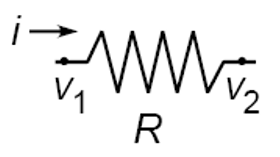
\includegraphics[width=\textwidth]{Resistor.png}
\end{minipage}
\hspace{0.05\textwidth}
\begin{minipage}[t]{0.5\textwidth}\vspace{0pt}
    \[
    \begin{aligned}
        v_R &= iR \\
        i(t) &= \frac{1}{R}(v_1 - v_2) \\
        I(s) &= \frac{1}{R}(V_1 - V_2)
    \end{aligned}
    \]
    \end{minipage}
    \item \textbf{Capacitor}\\
    \begin{minipage}[t]{0.3\textwidth}\vspace{0pt}
    \centering
    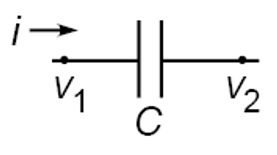
\includegraphics[width=\textwidth]{Capacitor.png}
    \end{minipage}
\hspace{0.15\textwidth}
    \begin{minipage}[t]{0.5\textwidth}\vspace{0pt}
    \[
    \begin{aligned}
        q &= Cv_c \\
        \frac{d}{dt}(q) &= \frac{d}{dt}(Cv_c) \quad \implies  \boxed{i(t) = C \frac{dv_C}{dt}} \\
        I(s) &= Cs(V_1 - V_2)
    \end{aligned}
    \]
    $I(s)$ comes from the Laplace transform of $i(t)$:
    \[i(t) = C\frac{d}{dt}(\underbrace{V_1-V_2}_{V_c})\]
    \end{minipage}
    \item \textbf{Inductor}\\
    \begin{minipage}[t]{0.3\textwidth}\vspace{0pt}
    \centering
    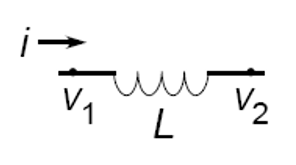
\includegraphics[width=\textwidth]{Inductor.png}
    \end{minipage}
\hspace{0.1\textwidth}
    \begin{minipage}[t]{0.5\textwidth}\vspace{0pt}
    \[
    \begin{aligned}
        v_L &= L \frac{di}{dt} \\
        i(t) &= i_o + \frac{1}{L} \int v_L(t) dt, \text{ zero IC} \\
        I(s) &= \frac{1}{Ls} (V_1 - V_2)
    \end{aligned}
    \]
    \end{minipage}
\end{itemize}
To write the equations of motion (characteristic equation) for an electrical system, we use Kirchhoff's current law (KCL) and Kirchhoff's voltage law (KVL) (see ESC 221 notes).
\section*{Impedance}
Impedance $Z$ is defined as the ratio of the voltage across an electrical element to the current through the element in the Laplace domain. Using impedance, every electrical element can be treated as a resistor, following an Ohm's law-like relationship:
\[Z = \frac{V(s)}{I(s)} \quad \implies i=\frac{v_1-v_2}{Z}, \quad v_1-v_2=iZ\]
The impedance of each element is as follows:
\begin{itemize}
    \item Resistor: $Z_R = R$
    \item Capacitor: $Z_C = \frac{1}{Cs}$
    \item Inductor: $Z_L = Ls$
\end{itemize}
\textbf{Summing Impedances}\\
Since we can treat every element as a resistor, we can sum impedances in series and parallel just like we would for resistors:
\begin{itemize}
    \item \textbf{Series Impedances}
\begin{center}
    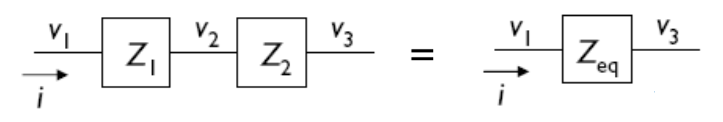
\includegraphics[width=0.6\textwidth]{Series Impedance.png}
\end{center}
    \[Z_\text{eq} = Z_1 + Z_2\]
    \item \textbf{Parallel Impedances}
\begin{center}
    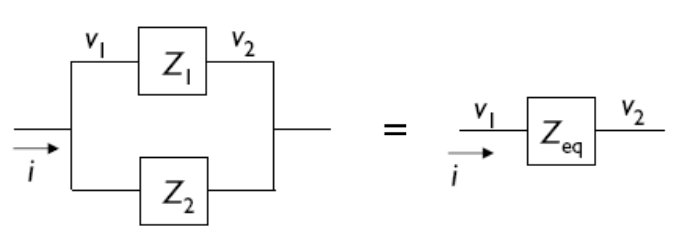
\includegraphics[width=0.6\textwidth]{Parallel Impedances.png}
\end{center}
    \[\frac{1}{Z_\text{eq}} = \frac{1}{Z_1} + \frac{1}{Z_2} \quad \implies \quad Z_\text{eq} = \frac{Z_1 Z_2}{Z_1 + Z_2}\]
\end{itemize}
\newpage\noindent
\textbf{Impedance Voltage Division}\\
Like the voltage division rule for resistors, we can also use the impedance to find the voltage across an element in a series circuit:
\begin{center}
    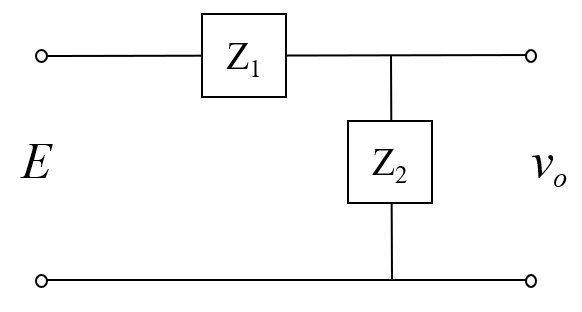
\includegraphics[width=0.5\textwidth]{Impedance Voltage Division.png}
\end{center}
\[v_o = \frac{Z_2}{Z_1 + Z_2} E\]
\underline{Note:} When writing the characteristic equation for an electrical system using impedances, we are in the Laplace domain, \textit{not the time domain}! This is often easier, though nodal and mesh analysis can also be used to write the equations of motion in the time domain.
\section*{Electrical and Mechanical Analogous Systems}
\begin{center}
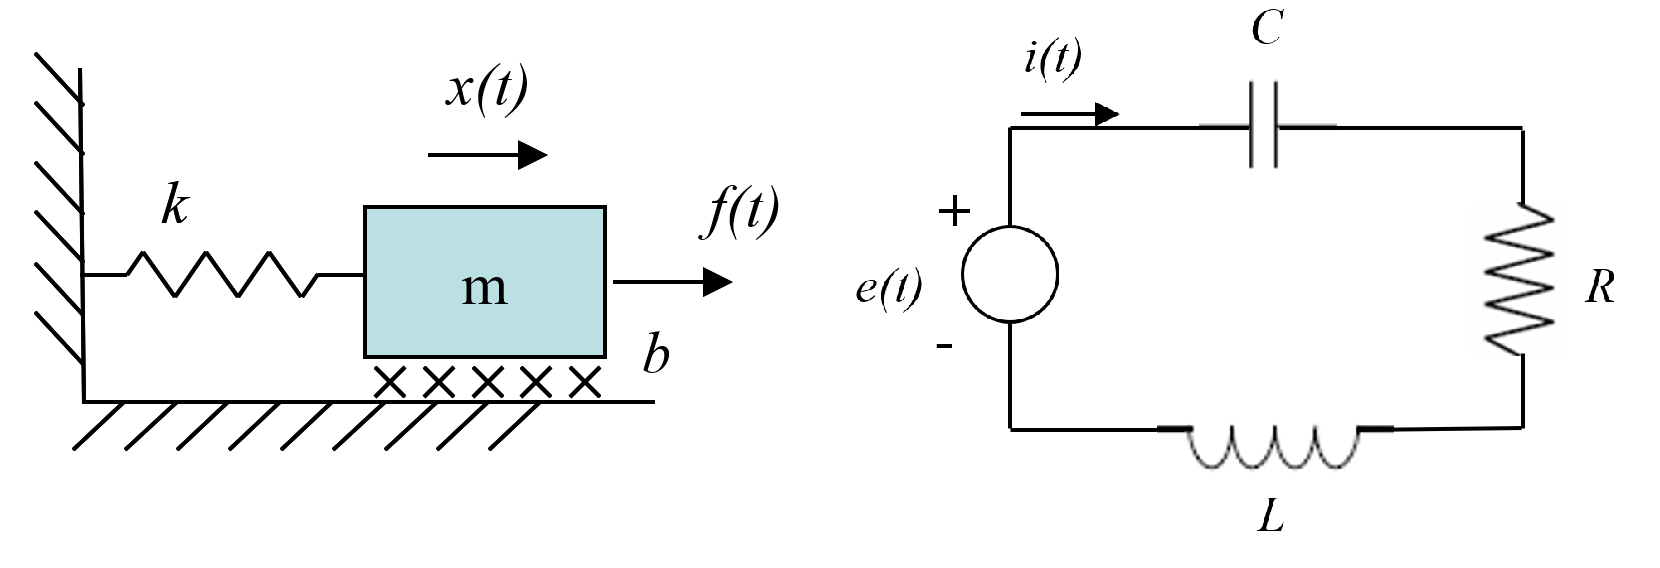
\includegraphics[width=0.7\textwidth]{Mechanical-Electrical Analogy.png}
\end{center}
Looking at the characteristic equations for the damped mass-spring system and the RLC circuit, we can see that they have the same form:
\[M\frac{d^2x}{dt^2} + b\frac{dx}{dt} + kx = f(t)\]
\[L\frac{d^2q}{dt^2} + R\frac{dq}{dt} + \frac{1}{C}q = e(t)\]
\textbf{Power}\\
Like mechanical systems, we can also define power for electrical systems as the product of effort $\times$ flow:
\[\begin{aligned}
P &= v \cdot i \\
&= \tau \cdot \omega \quad \text{(for rotational mechanical systems)} \\
&= F \cdot v \quad \text{(for translational mechanical systems)}
\end{aligned}\]
\newpage
\section*{Electromechanical Systems (DC Motor)}
The most common type of electromechanical system is a DC motor, which converts current to torque. It is commonly modeled as follows:
\begin{center}
    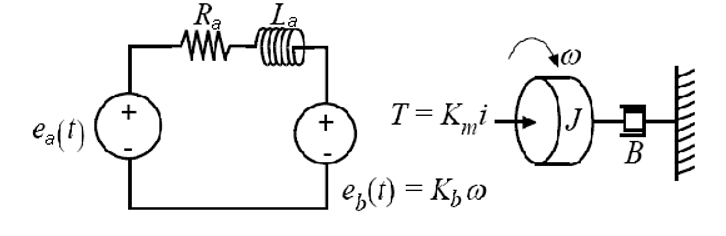
\includegraphics[width=0.8\textwidth]{DC Motor.png}
\end{center}
Where:
\[\begin{aligned}
R_a &= \text{armature resistance } (\Omega) \\
L_a &= \text{armature inductance } (\text{H}) \\
i_a &= \text{armature current } (\text{A}) \\
e_a &= \text{applied armature voltage } (\text{V}) \\
e_b &= \text{back emf (voltage produced by rotating armature) } (\text{V}) \\
\theta &= \text{angular displacement of motor shaft } (\text{rad}) \\
\omega &= \text{angular velocity of motor shaft } (\text{rad/s}) \\
T &= \text{torque developed by motor } (\text{N-m}) \\
J &= \text{moment of inertia of motor } (\text{kg-m}^2) \\
B &= \text{viscous friction coefficient of motor load } (\text{N-s/m or kg/s}) \\
K_m &= \text{motor torque constant (relates torque produced by electric part)} \\
K_b &= \text{back emf or generator constant (relates voltage induced by motion)}
\end{aligned}\]
The inertia term $J$ describes the inertia of the motor itself, typically if we are modeling a motor connected to some additional load, we will need to add the inertia of the load to $J$ (if it is a \textit{rigid} connection to the motor shaft). However, the load can be connected via a gear train or a flexible shaft, in which case we will need to draw out the FBDs to determine the equations of motion.\\\\
Like mentioned before, this is a 2 DOF system since the electrical and mechanical parts are coupled, so we will have to perform substitutions to find the transfer functions.
\[e_a - R_a i - L_a \frac{di}{dt} -K_b\omega= 0 \quad \text{(KVL)}\]
\[\sum \tau = J \frac{d\omega}{dt} = K_m i - B\omega \quad \text{(Newton)}\]
\[\implies \frac{\Omega(s)}{E_a(s)} = \frac{K_m}{(L_a s+R_a)(Js + B) + K_m K_b} \quad \text{(Transfer Function)}\]
\newpage
\section*{DC Motor Specs \& Characterization}
\begin{itemize}
    \item \textbf{DC Gain ($K$)}\\
    By definition, the DC gain is the gain of the system at \textit{steady state}. Therefore, time varying terms will go to zero:
    \[\frac{di}{dt} =0, \quad \frac{d\omega}{dt}=0\]
    In the transfer function (Laplace domain), this corresponds to $s=0$ (essentially just applying the final value theorem for a unit step input):
    \[K = \frac{K_m}{R_a B + K_m K_b}\]
    Finally, by setting $B=0$, we find the ideal max DC gain of the motor without any load/friction:
    \[K=\frac{1}{K_b}\]
    \item \textbf{Electrical Time Constant ($\tau_\text{elec}$)}\\
    Suppose we apply a \textit{brake} to the motor shaft so that $\omega=0$ and thus $e_b=0$, then the electrical time constant describes how fast the current (and thus torque by $T = K_m i$) reaches steady state. Rewriting the KVL equation with $\omega=0$ gives:
    \[e_a - R_a i - L_a \frac{di}{dt} = 0, \quad i=\frac{T}{K_m}\]
    \[\implies e_a - R_a \frac{T}{K_m} - L_a \frac{d}{dt}\left(\frac{T}{K_m}\right) = 0\]
    \[\implies \frac{T(s)}{E_a(s)} = \frac{K_m}{L_a s + R_a}\]
    \[\tau_\text{elec} = \frac{L_a}{R_a}\]
    \item \textbf{Mechanical Time Constant ($\tau_\text{mech}$)}\\
    Suppose the motor is allowed to freely spin down from some initial speed with zero applied voltage (free response) and set $B=0$, $L=0$. Rewriting the transfer function gives:
    \[\frac{\Omega(s)}{E_a(s)} = \frac{K_m}{R_aJs + K_m K_b}\]
    \[\tau_\text{mech} = \frac{R_aJ}{K_m K_b}\]
    This describes how fast an applied torque (or lack of) changes the speed of the motor, in terms of inertia and friction.
\end{itemize}
\underline{Note:} If we substitute known values into the general $\Omega(s)/E_a(s)$ transfer function, the slower pole corresponds to the mechanical time constant and the faster pole corresponds to the electrical time constant. This is because the electrical response results in a much faster transient response that decays to zero.\\\\
Rewriting the KVL equation at steady state ($di/dt=0, \,d\omega/dt=0$) gives us a way to relate the torque and applied voltage at steady state. Using this, we can determine the no load speed and stall torque of the motor.
\[e_a - R_a i -K_b\omega= 0 , \quad i=\frac{T}{K_m}\]
\[\implies e_a - R_a \frac{T}{K_m} - K_b\omega = 0\]
\begin{itemize}
    \item \textbf{No Load Speed ($T=0$)}\\
    The no load speed is the max speed ($\omega$) of the motor such that the back emf $e_b$ is equal to the applied voltage $e_a$, which means that there is no current flowing through the motor and thus no torque produced. Setting $T=0$ gives:
    \[\omega_\text{no load} = \frac{e_a}{K_b}\]
    \item \textbf{Stall Torque ($\omega=0$)}\\
    Stall torque is the max torque ($T$) generated by the motor when it is stopped ($\omega=0$), thus there is no back emf and the current is at its max. Setting $\omega=0$ gives:
    \[T_\text{stall} = \frac{K_m}{R_a} e_a\]
\end{itemize}
\underline{Note:} These formulas are NOT general, they only apply to the specific DC motor model shown above. If we have a different set-up with gears, shafts, or a load, then we will need to repeat these processes with the new equations of motion to characterize the DC motor system.
\section*{Gears}
\begin{minipage}[t]{0.5\textwidth}\vspace{0pt}
\centering
    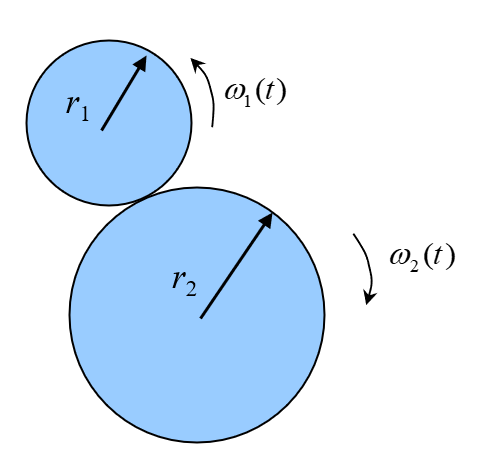
\includegraphics[width=\textwidth]{Gear Ratio.png} 
\end{minipage}
\hfill
\begin{minipage}[t]{0.5\textwidth}\vspace{0pt}
Gear ratios can be defined in terms of the number of teeth on each gear or the radius of each gear:
\[\text{Gear ratio} = \frac{N_2}{N_1} = \frac{r_2}{r_1}\]
Where $N$ is the number of teeth and $r$ is the radius of the gear. They mean the same thing since the number of teeth is proportional to the radius of the gear (same tooth size/module).
\end{minipage}\\\\
Since the gears rotate without slipping, the relative velocity at the contact point is zero, following the sign convention in the diagram above, we can say that
\[r_1 \omega_1 = r_2 \omega_2 \quad \implies \frac{\omega_2}{\omega_1}=\frac{r_1}{r_2}=\frac{N_1}{N_2}\]
Neglecting friction loss, the torque is also related by the gear ratio:
\[\tau_1 \omega_1 = \tau_2 \omega_2 \quad \implies \frac{\tau_2}{\tau_1}=\frac{\omega_1}{\omega_2}=\frac{N_2}{N_1}\]
\underline{Note:} It is best to draw the internal reaction forces between the gears to determine the direction of the torques in the FBD and resulting equations of motion for each gear.
\vspace{1em}
\noindent\hrule
\vspace{1em}
\newpage
\begin{center}
{\LARGE State Space Representation\par}
\end{center}
We are able to rewrite the equations of motion of a system in the time domain into a matrix form using state variables. This is useful because it allows us to write an n-th order system as a system of n first order equations.
\begin{itemize}
    \item \textbf{State Variables}\\
    State variables are a set of variables that completely describes the behavior of the system along with the input.
    \item \textbf{State Vector}\\
    The state vector is a column vector containing all the state variables.
\end{itemize}
The state space representation of a system is given by the following form:
\[\begin{aligned}
\dot{\underline{x}} &= [A]{\underline{x}} + [B]\underline{u} \\
\underline{y} &= [C]{\underline{x}} + [D]\underline{u}
\end{aligned}\]
Where:
\begin{itemize}
    \item $\underline{x}$ = state vector
    \item $\underline{u}$ = input vector
    \item $\underline{y}$ = output vector
    \item $[A]$ = state matrix
    \item $[B]$ = input matrix
    \item $[C]$ = output matrix
    \item $[D]$ = direct transition matrix (output related to input)
\end{itemize}
Starting from the equations of motion and the defined state variables, we can rewrite the equations of motion in terms of the state variables. Ensure that the matrix multiplication (dot product between rows and columns) correctly reproduces the rewritten equations of motion and that the dimensions are consistent.\\\\
The output matrix is often either a matrix that selects certain state variables as outputs, or a matrix that operates on the state variables to produce the output (ie. momentum is a velocity state variable multiplied by mass). The direct transmission matrix is often zero, but it can be non-zero if the output is directly related to the input (ie. if the output is the input voltage in an electrical system).
\section*{Transfer Function Matrices}
Like how we can derive transfer functions in the Laplace domain from the equations of motion, we can do the same in state space representation using matrix arithmetic. Starting with:
\[\begin{aligned}
\dot{\underline{x}} &= [A]{\underline{x}} + [B]\underline{u} \\
\underline{y} &= [C]{\underline{x}} + [D]\underline{u}
\end{aligned}\]
Taking the Laplace transform:
\[\begin{aligned}
    s\underline{X} &= [A]\underline{X} + [B]\underline{U} \\
     \underline{Y} &= [C]\underline{X} + [D]\underline{U}
\end{aligned}\]
Isolate the State Vector ($\underline{X}$):
\[\underline{X} = [sI - A]^{-1}[B]\underline{U}\]
Substitute $\underline{X}$ into the Output Equation:
\[\underline{Y} = [C]\underbrace{\left( [sI - A]^{-1}[B]\underline{U} \right)}_{\text{Sub for } \underline{X}} + [D]\underline{U}\]
Factor out $\underline{U}$ for the Transfer Function:
\[\boxed{\frac{\underline{Y}}{\underline{U}} = [C][sI - A]^{-1}[B] + [D]}\]
\underline{Recall:} We can invert a 2x2 matrix using the formula:
\[
A =
\begin{pmatrix}
a & b \\
c & d
\end{pmatrix}\]
\[A^{-1} = \frac{1}{ad - bc}
\begin{pmatrix}
d & -b \\
-c & a
\end{pmatrix},
\quad \text{if } ad - bc \neq 0.\]
\vspace{1em}
\noindent\hrule
\vspace{1em}
\newpage
\begin{center}
{\LARGE Block Diagrams\par}
\end{center}
\section*{Block Diagram Elements}
\begin{itemize}
    \item \textbf{Signals}: time varying quantities (ex: $u(t), y(t)$) that represent inputs and outputs of the system. Inputs are represented as arrows pointing into the system, while outputs are represented as arrows pointing out of the system.
    \begin{center}
    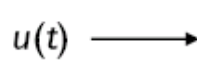
\includegraphics[width=0.15\textwidth]{Signal.png}
    \end{center}
    \item \textbf{Systems}: represent differential equations that relate inputs to outputs, often represented as blocks containing the transfer function of the system (ex: $H(s)=\frac{Y(s)}{U(s)}$).
    \begin{center}
    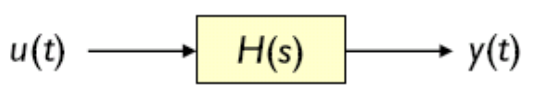
\includegraphics[width=0.45\textwidth]{Block Diagram.png}
    \end{center}
    \[Y(s) = H(s)U(s)\]
    \item \textbf{Summing Junctions}: adds together signals with sign indicated by the arrowheads. Signals can be added together in both the time domain and the Laplace domain.
    \begin{center}
    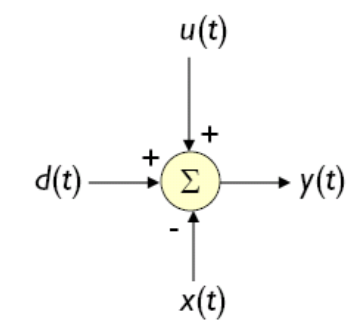
\includegraphics[width=0.25\textwidth]{Summing Junction.png}
    \end{center}
    \[y(t) = u(t) +d(t)-x(t) \implies Y(s) = U(s)+D(s)-X(s)\]
\end{itemize}
\newpage
\section*{Control Systems (Closed Loop Transfer Function)}
To reduce the effect of unwanted inputs such as disturbances and noise, we can use feedback control to create a closed loop system. The block diagram for a closed loop system is as follows:
\begin{center}
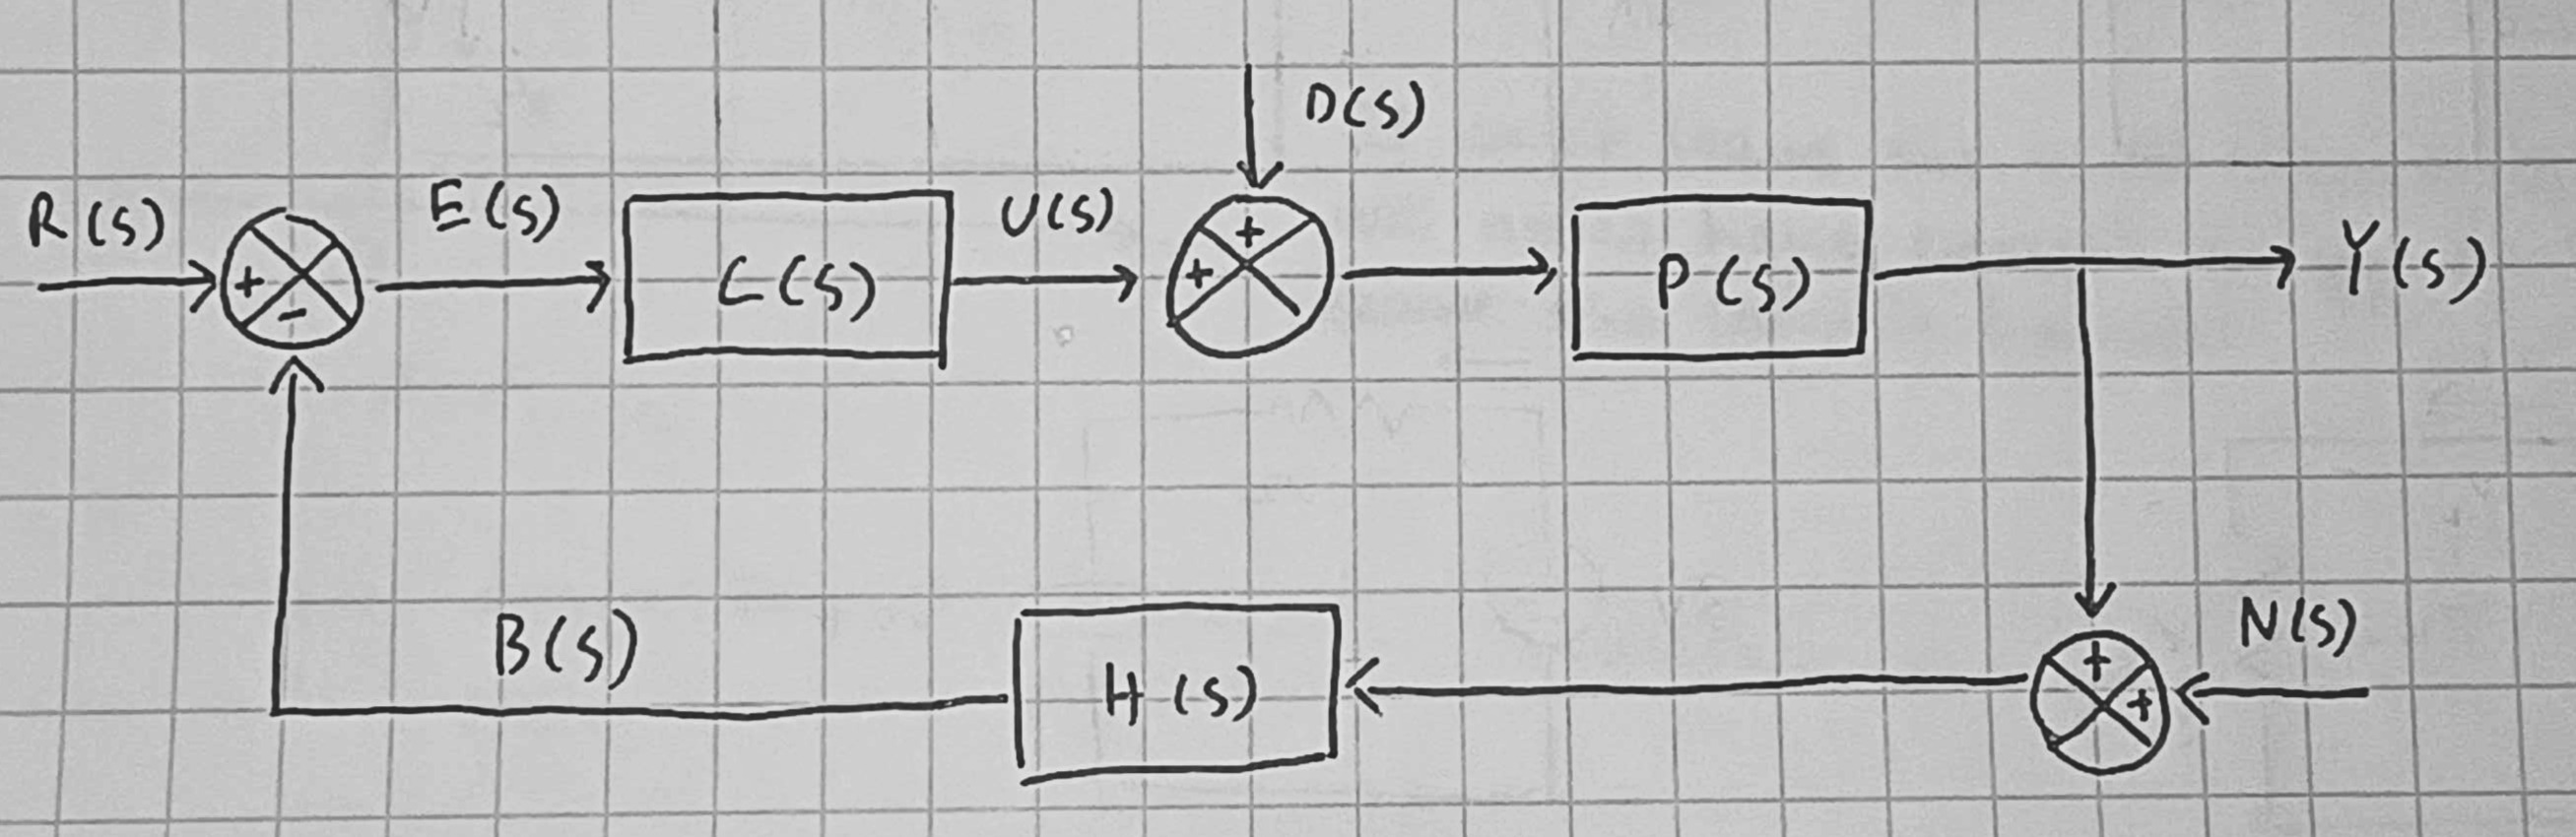
\includegraphics[width=0.7\textwidth]{CLTF.jpg}
\end{center}
Where:
\begin{itemize}
    \item $C(s)$: controller transfer function (ex: PID controller)
    \item $P(s)$: plant transfer function representing the system we want to control (ex: DC motor)
    \item $H(s)$: feedback transfer function (for \textbf{unity feedback}, $H(s)=1$)
\end{itemize}
Here, we have multiple inputs:
\begin{itemize}
    \item $R(s)$: reference input (desired output value)
    \item $D(s)$: disturbance input (unwanted input that affects the system)
    \item $N(s)$: noise input (unwanted input that affects the measurement of the output)
\end{itemize}
Additionally, in between the elements we have the following signals:
\begin{itemize}
    \item $E(s)$: error signal (difference between reference input and feedback)
    \item $U(s)$: controller output signal
    \item $B(s)$: feedback signal (output fed back into the system)
    \item $Y(s)$: output signal
\end{itemize}
\textbf{Transfer Functions}\\
Note that since we have multiple inputs, we can derive the transfer function for each input by using \textbf{superposition} (isolate a single input and set all other inputs to zero).\\\\
In addition to typical transfer functions that relate the outputs to inputs we define the following vocabulary for control system transfer functions:
\begin{itemize}
    \item \textbf{Open Loop Transfer Function}: product of the transfer functions around the loop
    \[\frac{B(s)}{E(s)}=C(s)P(s)H(s)\]
    \item \textbf{Feedforward Transfer Function}: product of the transfer functions along the forward path
    \[\frac{Y(s)}{E(s)}=C(s)P(s)\]
    \item \textbf{Closed Loop Transfer Function}: relates the output to the reference input
    \[\boxed{\frac{Y(s)}{R(s)} = \frac{C(s)P(s)}{1 \pm  C(s)P(s)H(s)} = \frac{\text{(Feedforward TF)}}{1 \pm \text{(Open Loop TF)}}}\]
\end{itemize}
\underline{Note:} The $\pm$ in the closed loop transfer function depends on the sign of the feedback (positive or negative feedback). For negative feedback (subtracting the feedback signal), we use the plus sign; for positive feedback, we use the minus sign.\\\\
\underline{Recall DC Gain:} Like before, the DC gain is defined as the steady state output given a unit step input, and we can find the DC gain using the various transfer functions we have derived for the system and final value theorem.
\textbf{Types of Control Systems}\\
\begin{itemize}
    \item \textbf{Closed-loop system:} transfer function from reference input to output
    \item \textbf{Open-loop system:} transfer function without feedback
    \begin{center}
    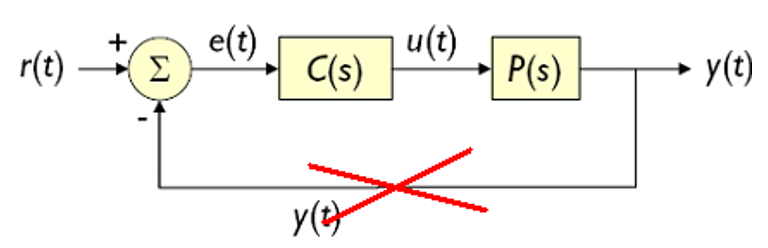
\includegraphics[width=0.5\textwidth]{Feedforward.png}
    \end{center}
\end{itemize}
\section*{Block Diagram Algebra and Simplification}
When simplifying block diagrams, we can look at the nodes between groups of blocks and rewrite the groups using their equivalent transfer function.\\\\
\textbf{Blocks in series}: multiply the transfer functions
\begin{center}
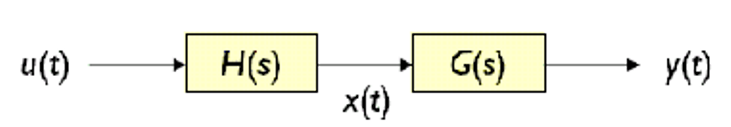
\includegraphics[width=0.5\textwidth]{Blocks in series.png}
\end{center}
\[X(s)=H(s)U(s),\quad Y(s)=G(s)X(s)\]
\[\implies \frac{Y(s)}{U(s)} = G(s)H(s)\]
\newpage\noindent
Thus simplified block diagram:
\begin{center}
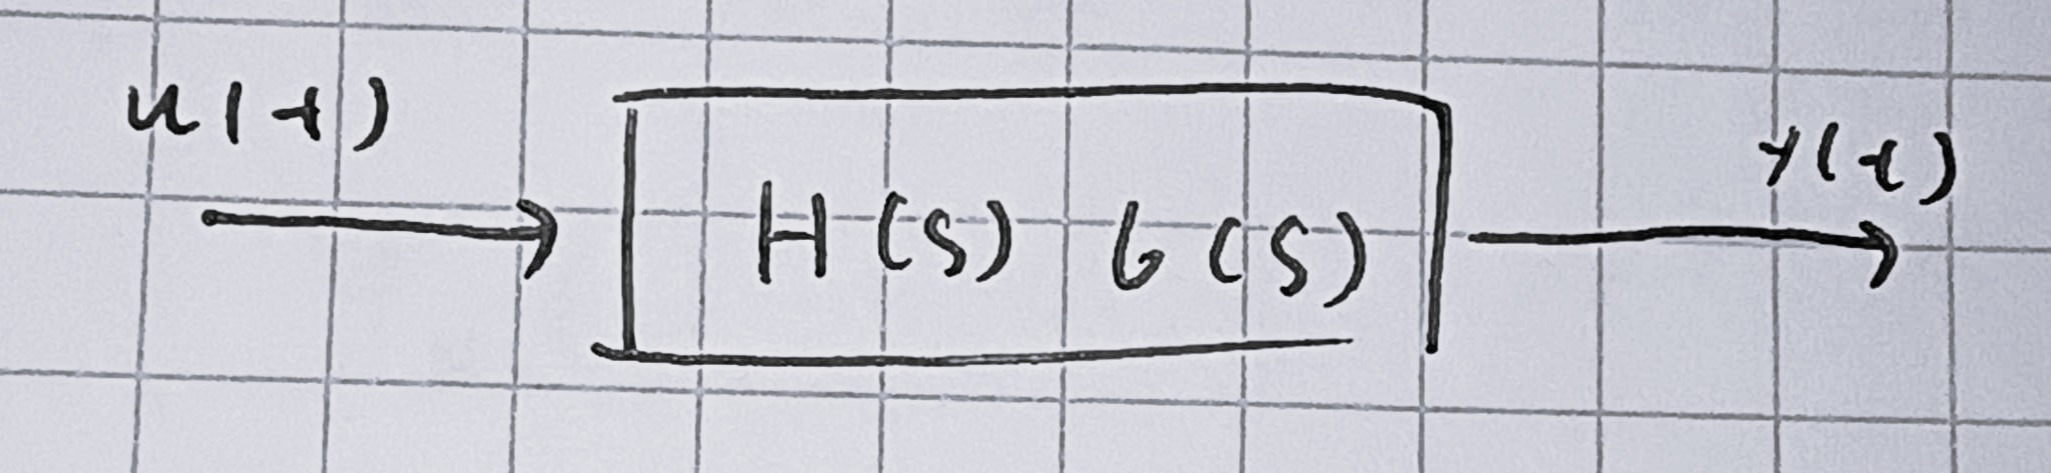
\includegraphics[width=0.5\textwidth]{Series blocks.jpg}
\end{center}
\textbf{Blocks in parallel}: add the transfer functions
\begin{center}
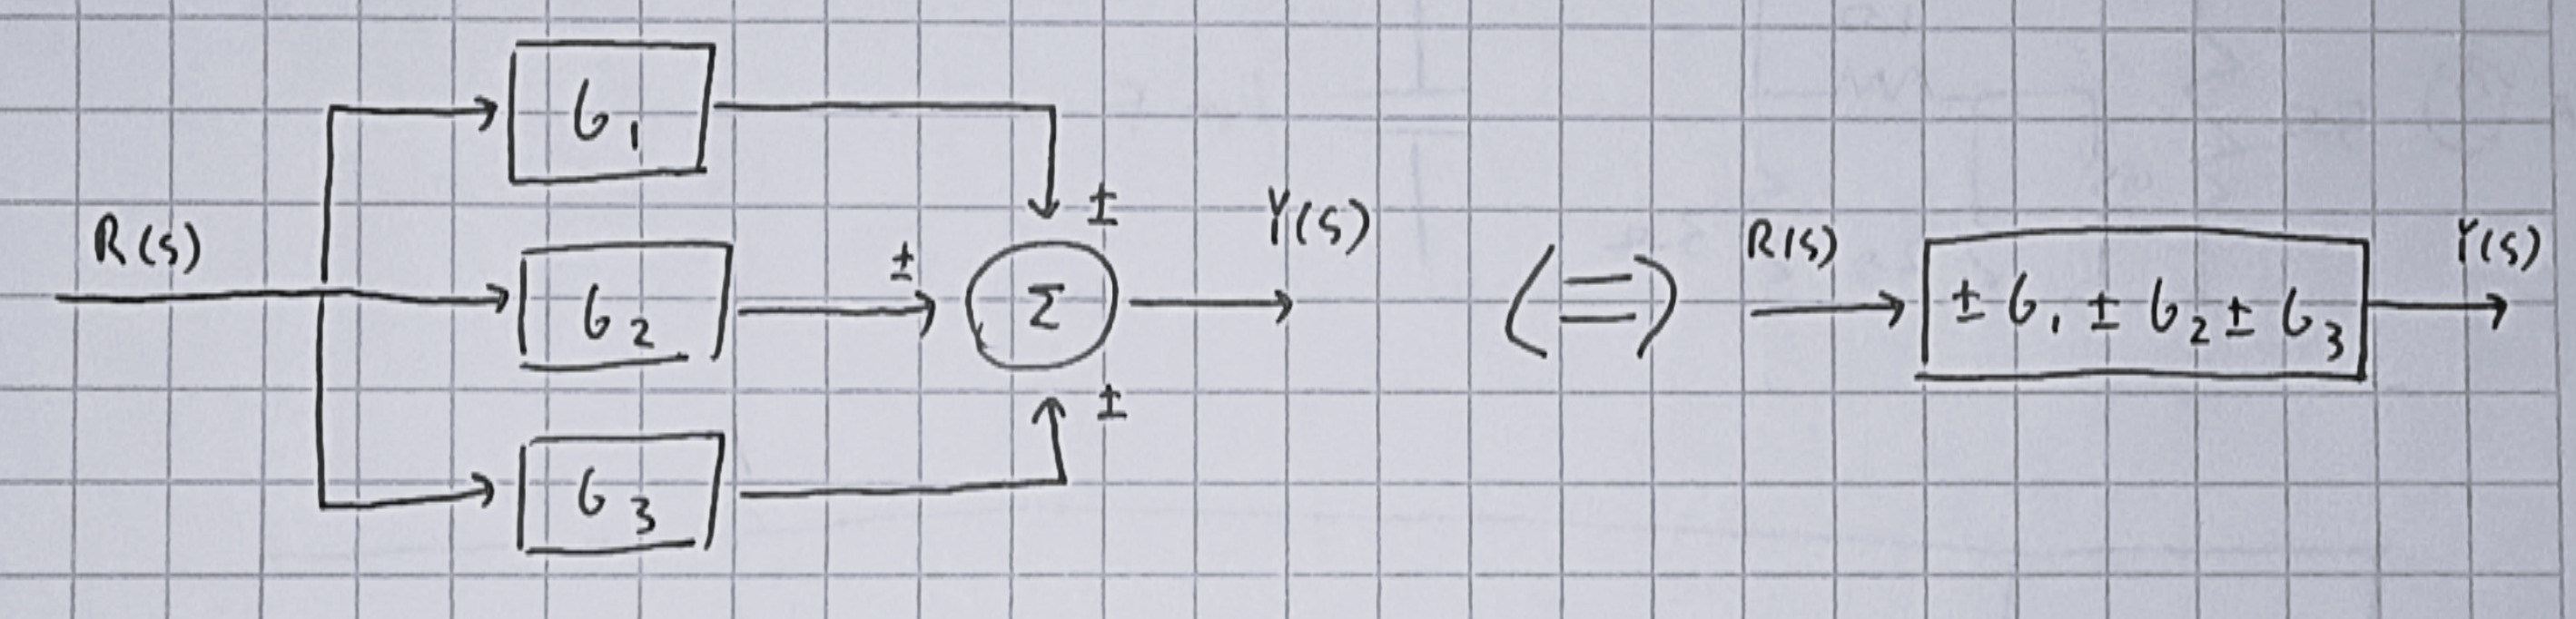
\includegraphics[width=0.8\textwidth]{Parallel blocks.jpg}
\end{center}
\textbf{General feedback loops}: use the closed loop transfer function
\begin{center}
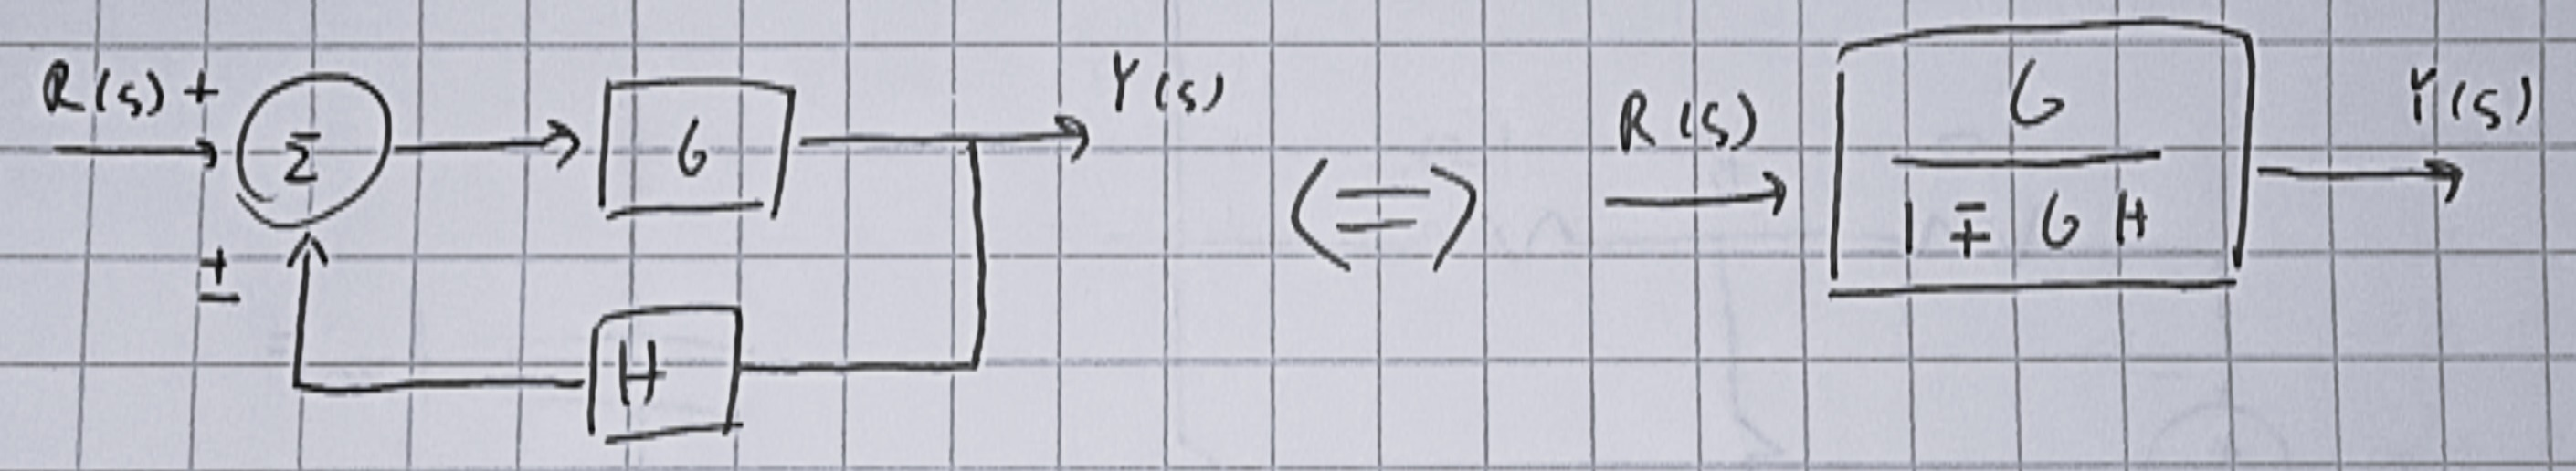
\includegraphics[width=0.8\textwidth]{Feedback.jpg}
\end{center}
In addition to these simplifications, we can manipulate the block diagram by moving blocks according to block diagram algebra in the following ways:\\\\
\textbf{Rule 1}
\begin{center}
    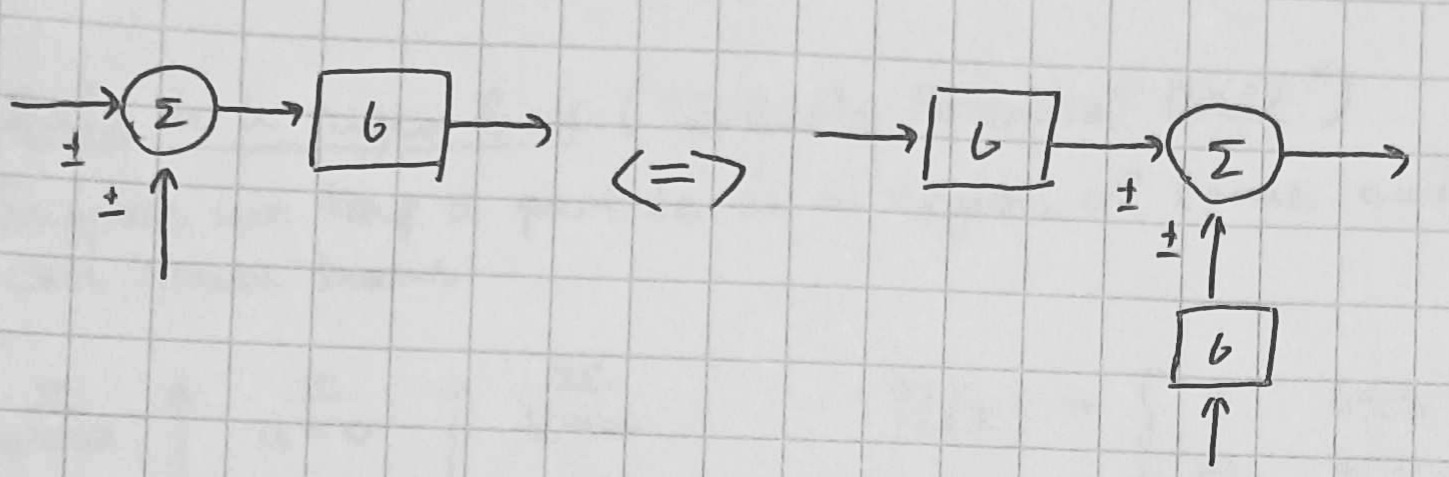
\includegraphics[width=0.6\textwidth]{Rule 1.jpg}
    \end{center}
\textbf{Rule 2}
\begin{center}
    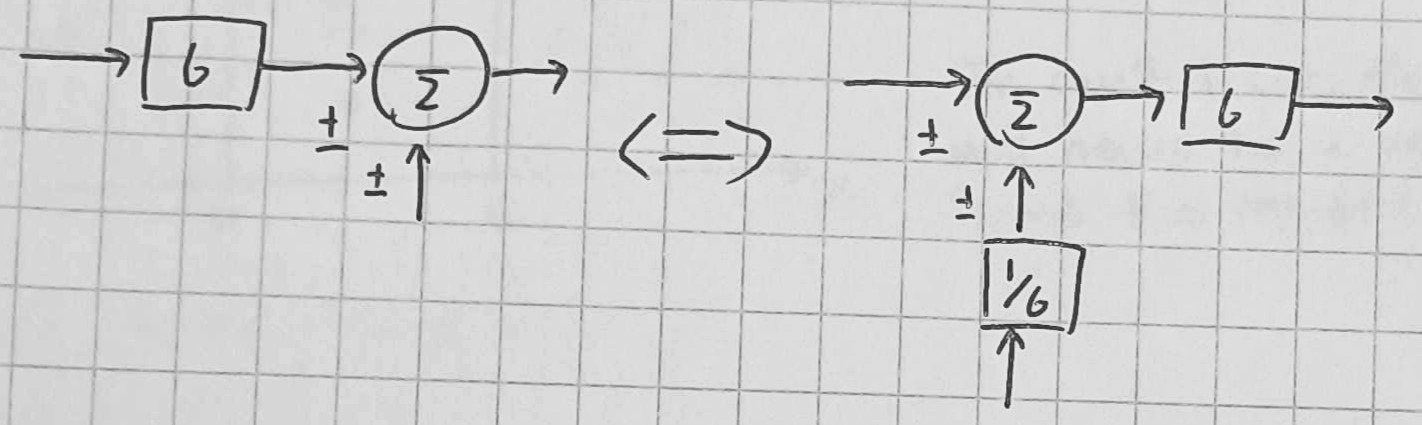
\includegraphics[width=0.6\textwidth]{Rule 2.jpg}
    \end{center}
\textbf{Rule 3}
\begin{center}
    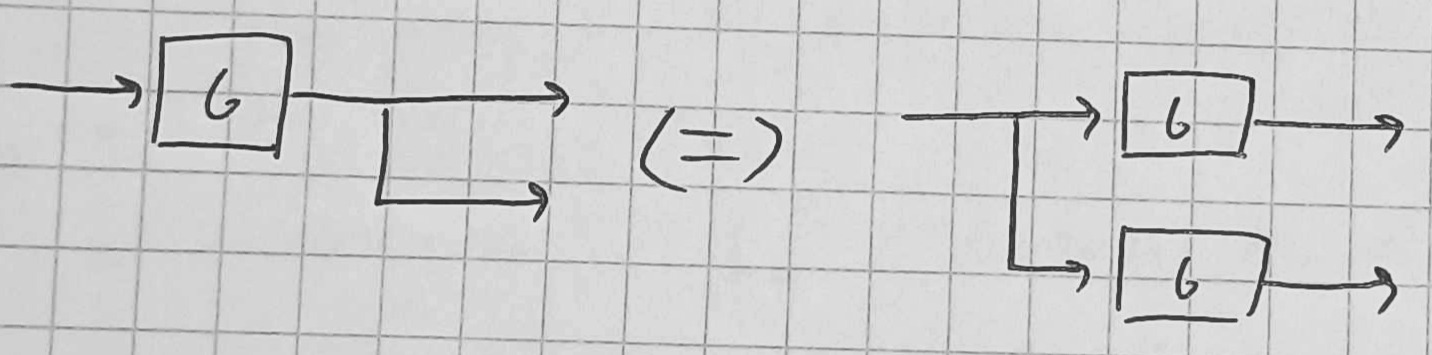
\includegraphics[width=0.6\textwidth]{Rule 3.jpg}
    \end{center}
    \newpage\noindent
\textbf{Rule 4}
\begin{center}
    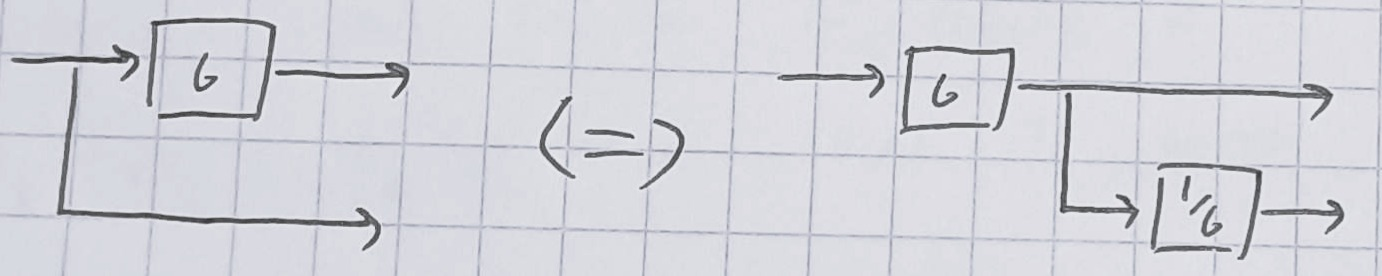
\includegraphics[width=0.6\textwidth]{Rule 4.jpg}
    \end{center}
\textbf{Rule 5}
\begin{center}
    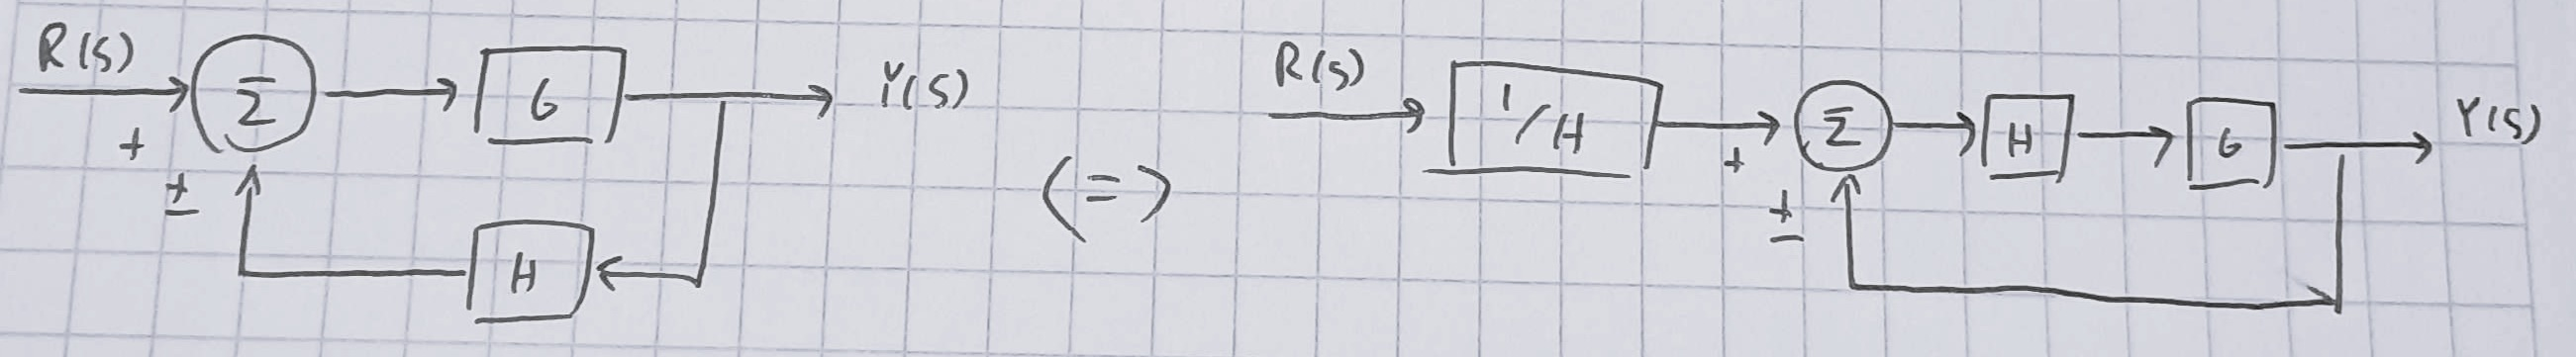
\includegraphics[width=1\textwidth]{Rule 5.jpg}
    \end{center}
\section*{Block Diagram for a linear system represented in state space}
\begin{center}
\includegraphics[width=0.8\textwidth]{State Space Block Diagram.png}
\end{center}
\begin{itemize}
    \item[Step 1:] Draw $n$ integrator ($s^{-1}$) blocks, and assign a state variable to the output of each block.
    \item[Step 2:] At the input to each block (which represents the derivative of its state variable) draw a summing element.
    \item[Step 3:] Use the state equations to connect the state variables and inputs to the summing elements through scaling operator blocks.
    \item[Step 4:] Expand the output equations and sum the state variables and inputs through a set of scaling operators to form the components of the output.
\end{itemize}
\newpage
\section*{Block Diagram for a linear system represented as an ODE}
Simulink model:
\begin{center}
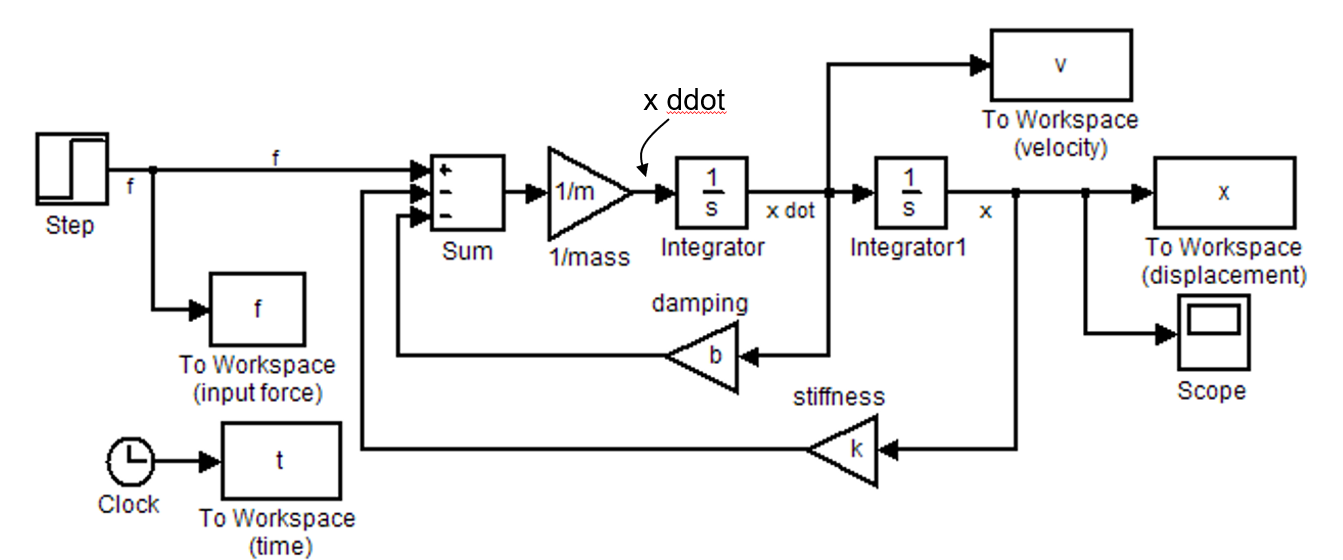
\includegraphics[width=0.8\textwidth]{ODE Block Diagram.png}
\end{center}
\vspace{-1em}
\[m\ddot{x}+b\dot{x}+kx=f(t)\]
\vspace{1em}
\noindent\hrule
\vspace{1em}
\newpage
\begin{center}
{\LARGE Linearization\par}
\end{center}
So far we have only dealt with linear systems, where the governing equations of the system are linear differential equations. However, the real world is non-linear. Thus, we will need to \textit{linearize} non-linear systems to be able to apply the linear system analysis techniques we have learned so far. Generally, we do this by approximating the \textit{local} behavior of a non-linear system around an equilibrium point (operating point) using the first order Taylor expansion.\\\\
Defining the operating point as $\bar{x}$ and the incremental variable as $\hat{x}$, we can see graphically how the linearization process works:
\[\boxed{x=\bar{x}+\hat{x},\quad f(\hat{x}) = f(x)-f(\bar{x})}\]
\begin{center}
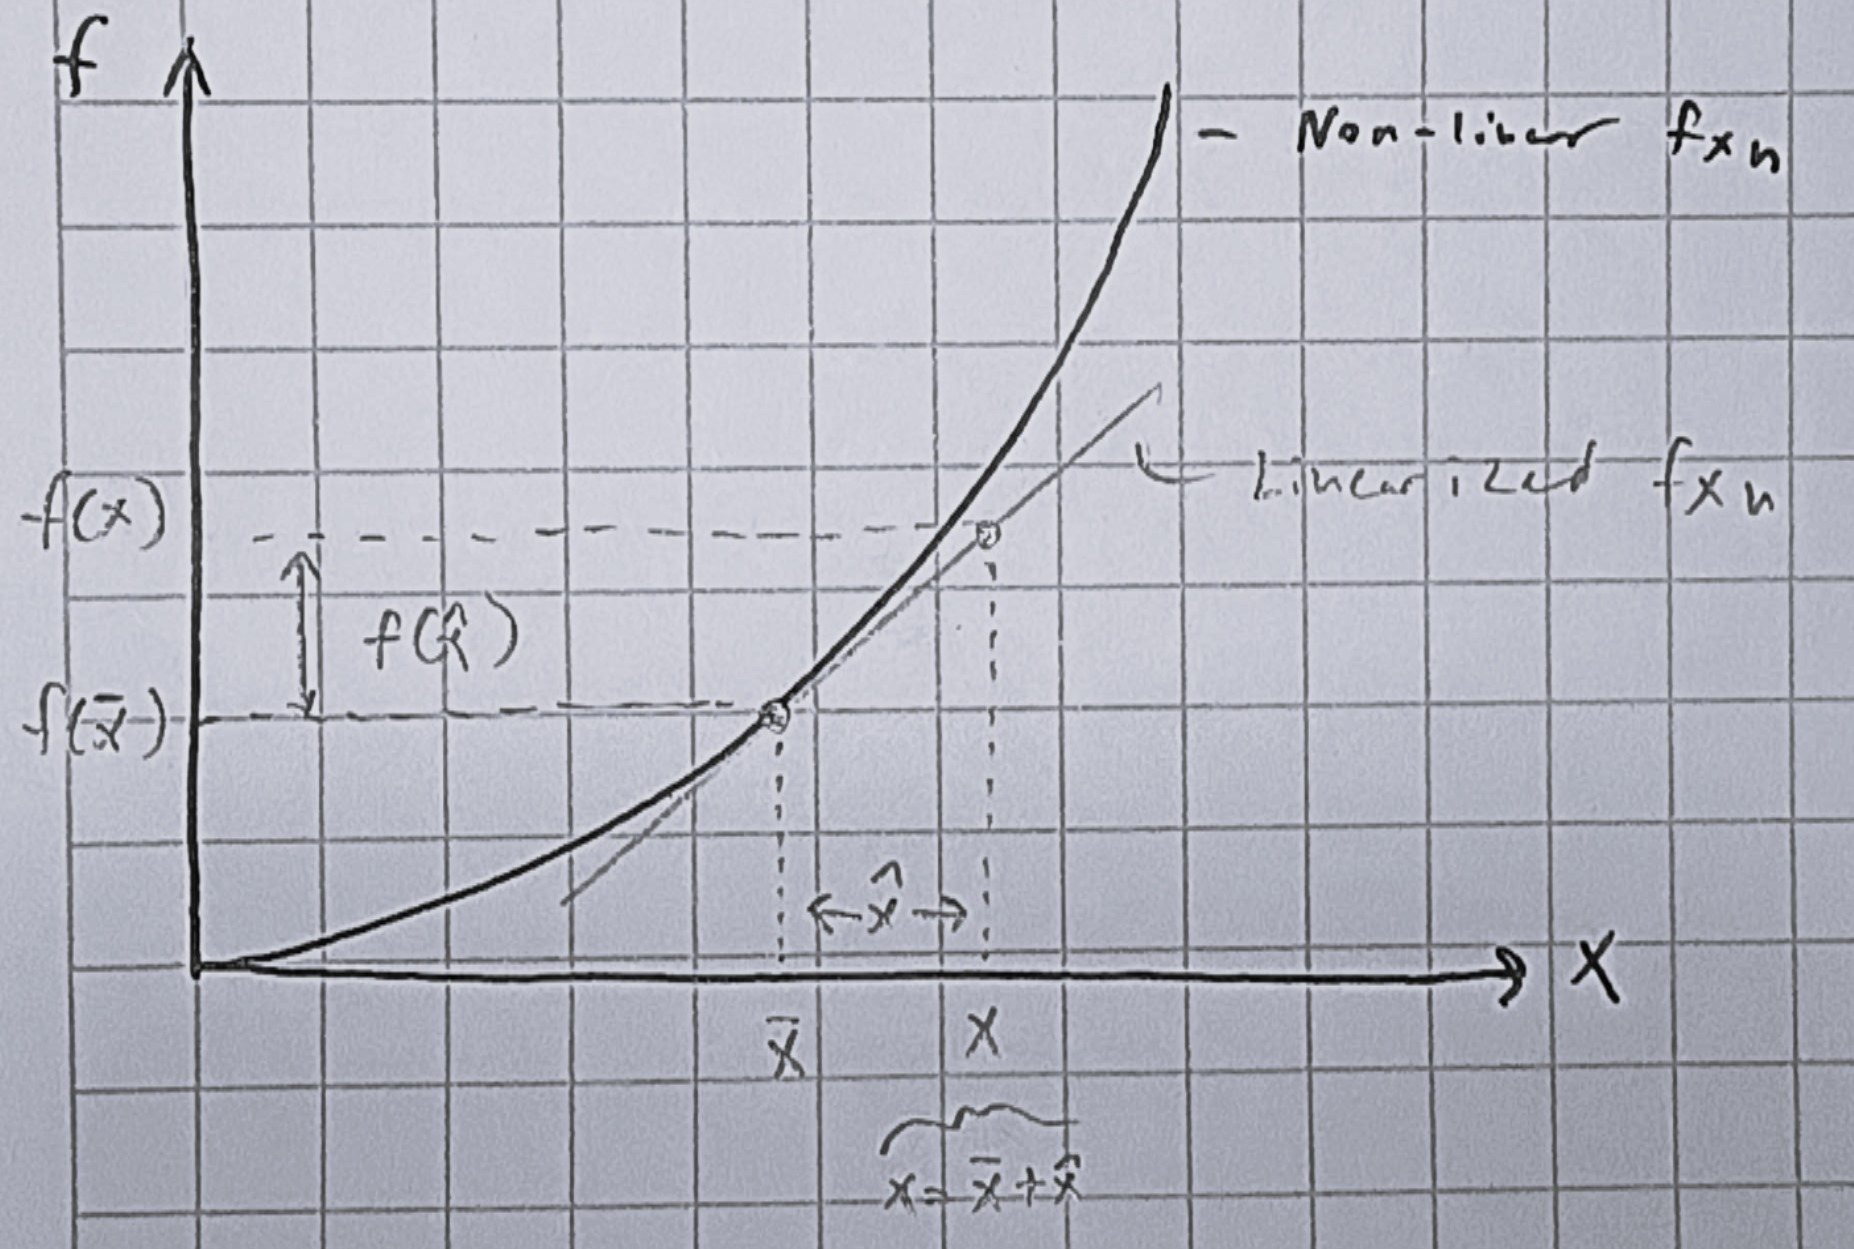
\includegraphics[width=0.7\textwidth]{Linearization.jpg}
\end{center}
Mathematically, approximating the non-linear function $f(x)$ around the operating point $\bar{x}$ gives us a tangent line that approximates the behavior of the system near $\bar{x}$:
\[k=\frac{df}{dx}\bigg|_{x=\bar{x}}\]
\[f(x) = f(\bar{x})+k(x-\bar{x})\]
Using the definition of $\hat{x}$, we can rewrite the linearized function in terms of the incremental variable $\hat{x}$:
\[f(x)=f(\bar{x})+k\hat{x}\quad \implies \quad \boxed{f(\hat{x})=k\hat{x}}\]
Now we are able to apply our techniques for linear systems to anaylze the behavior of the system under $\hat{x}$, however we must remember that the \textit{total} response of the system is given by
\[f(x) = f(\bar{x}) + f(\hat{x}),\quad x = \bar{x} + \hat{x} \]
Effectively, this linearization technique is like a transformation from the original $(x, f(x))$ coordinate system to a new $(\hat{x}, f(\hat{x}))$ coordinate system that is centered around the operating point $(\bar{x}, f(\bar{x}))$. So we need to remember to transform the results back to the original coordinate system when necessary.\\\\
\underline{Note:} The operating point is defined as the equilibrium point of the system since the further away from the operating point we are, the worse the linear approximation will be.
\section*{Linearization Procedure}
\begin{itemize}
    \item[I.] \textbf{Define operating point \& incremental variables:} \\
    Let $f(x)$ be a non-linear function of $x$, let $\bar{x}$ be the nominal operating point and let $\hat{x} = x - \bar{x}$ be the deviation from the operating point. Linearize $f(x)$ using Taylor series or graphical method.
    
    \item[II.] \textbf{Find operating point:} \\
    To find the operating point, find the ""equilibrium"" solution of the system when $\bar{x} = (\text{constant})$ by setting $\dot{x} = \ddot{x}=0$.
    
    \item[III.] \textbf{Replace with linearized terms:} \\
    Replace the linearized $f(x)$ and $x = \hat{x} + \bar{x}$ (and $u = \hat{u} + \bar{u}$ if needed) in the non-linear differential equation.
\end{itemize}
The linearized equation is in terms of $\hat{x}$ (and $\hat{u}$ if it exists). This linearized equation describes the actual non-linear system close to the operating point. The further from the operating point, the less accurate the description is.
\noindent\hrule
\vspace{1em}
\newpage
\begin{center}
{\LARGE Fluid Systems\par}
\end{center}
In trying to model fluid systems, we try to find analogous definitions to electrical systems. For example:
\begin{itemize}
    \item \textbf{Fluid Resistance}: elements that generate resistance to fluid flow (ex: pipe, valve)
    \item \textbf{Fluid Capacitance}: elements that store fluid (ex: tank)
    \item \textbf{Fluid Inductance}: accounts for the kinetic energy of the fluid (usually negligible)
    \item \textbf{Source/Driving Force}: pressure or flow source (ex: pump)
\end{itemize}
\section*{Variables}
\begin{itemize}
    \item Pressure difference across an element
    \[p_{12}=p_1-p_2\quad\text{[N/m$^2$]}\]
    \item Volumetric flow rate through an element
    \[q \quad\text{[m$^3$/s]}\]
    \item Fluid power across an element (effort $\times$ flow) represents the rate of energy transfer through that element. Depending on the direction of flow and the pressure difference, this power can be either positive or negative (input/output). For example, a pump provides positive power (increases pressure), while a valve dissipates power (decreases pressure).
    \[P=qp_{12}\quad\text{[W]}\]
\end{itemize}
\section*{Fluid Resistance}
Fluid resistance ($R$) defines how difficult it is to push fluid at a certain flow rate through an element. Since fluid flow can be driven by either a pressure difference or a difference in fluid levels ("head"), there are two definitions for fluid resistance. To identify which case, check the units of the resistance given in the problem.\\\\
\textbf{Pressure difference}:\\
\[\text{Units:}\quad  \left[\frac{\text{N/m}^2}{\text{m}^3/\text{s}}\right] = \left[\frac{\text{N}\cdot\text{s}}{\text{m}^5}\right]\]
Although flow rate through an element has a non-linear relationship with pressure difference, we \textit{assume} a linear relationship for the purposes of modeling:
\[\boxed{p_{12} = Rq}\]
\underline{Note:} In reality, the relationship between pressure difference and flow rate is only linear for laminar flow, and becomes non-linear for turbulent flow.\\\\
This is similar to Ohm's law $V=IR$ for electrical systems. Like voltage difference, fluid flows from high pressure to low pressure, so the flow rate is positive when $p_1 > p_2$ and negative when $p_1 < p_2$ (\textbf{Sign Convention}).
\begin{center}
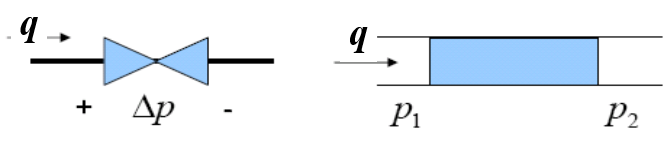
\includegraphics[width=0.5\textwidth]{Fluid R_p.png}
\end{center}
\underline{Note:} Typically we use \textit{gauge pressures} so atmospheric pressure is considered zero, be careful if the problem gives absolute pressures however.\\\\
\textbf{Head difference}:\\
\[\text{Units:}\quad \left[\frac{\text{m}}{\text{m}^3/\text{s}}\right] = \left[\frac{\text{s}}{\text{m}^2}\right]\]
Assuming a linear relationship between head difference and flow rate gives us:
\[\boxed{h_{12} = Rq}\]
For example:
\begin{center}
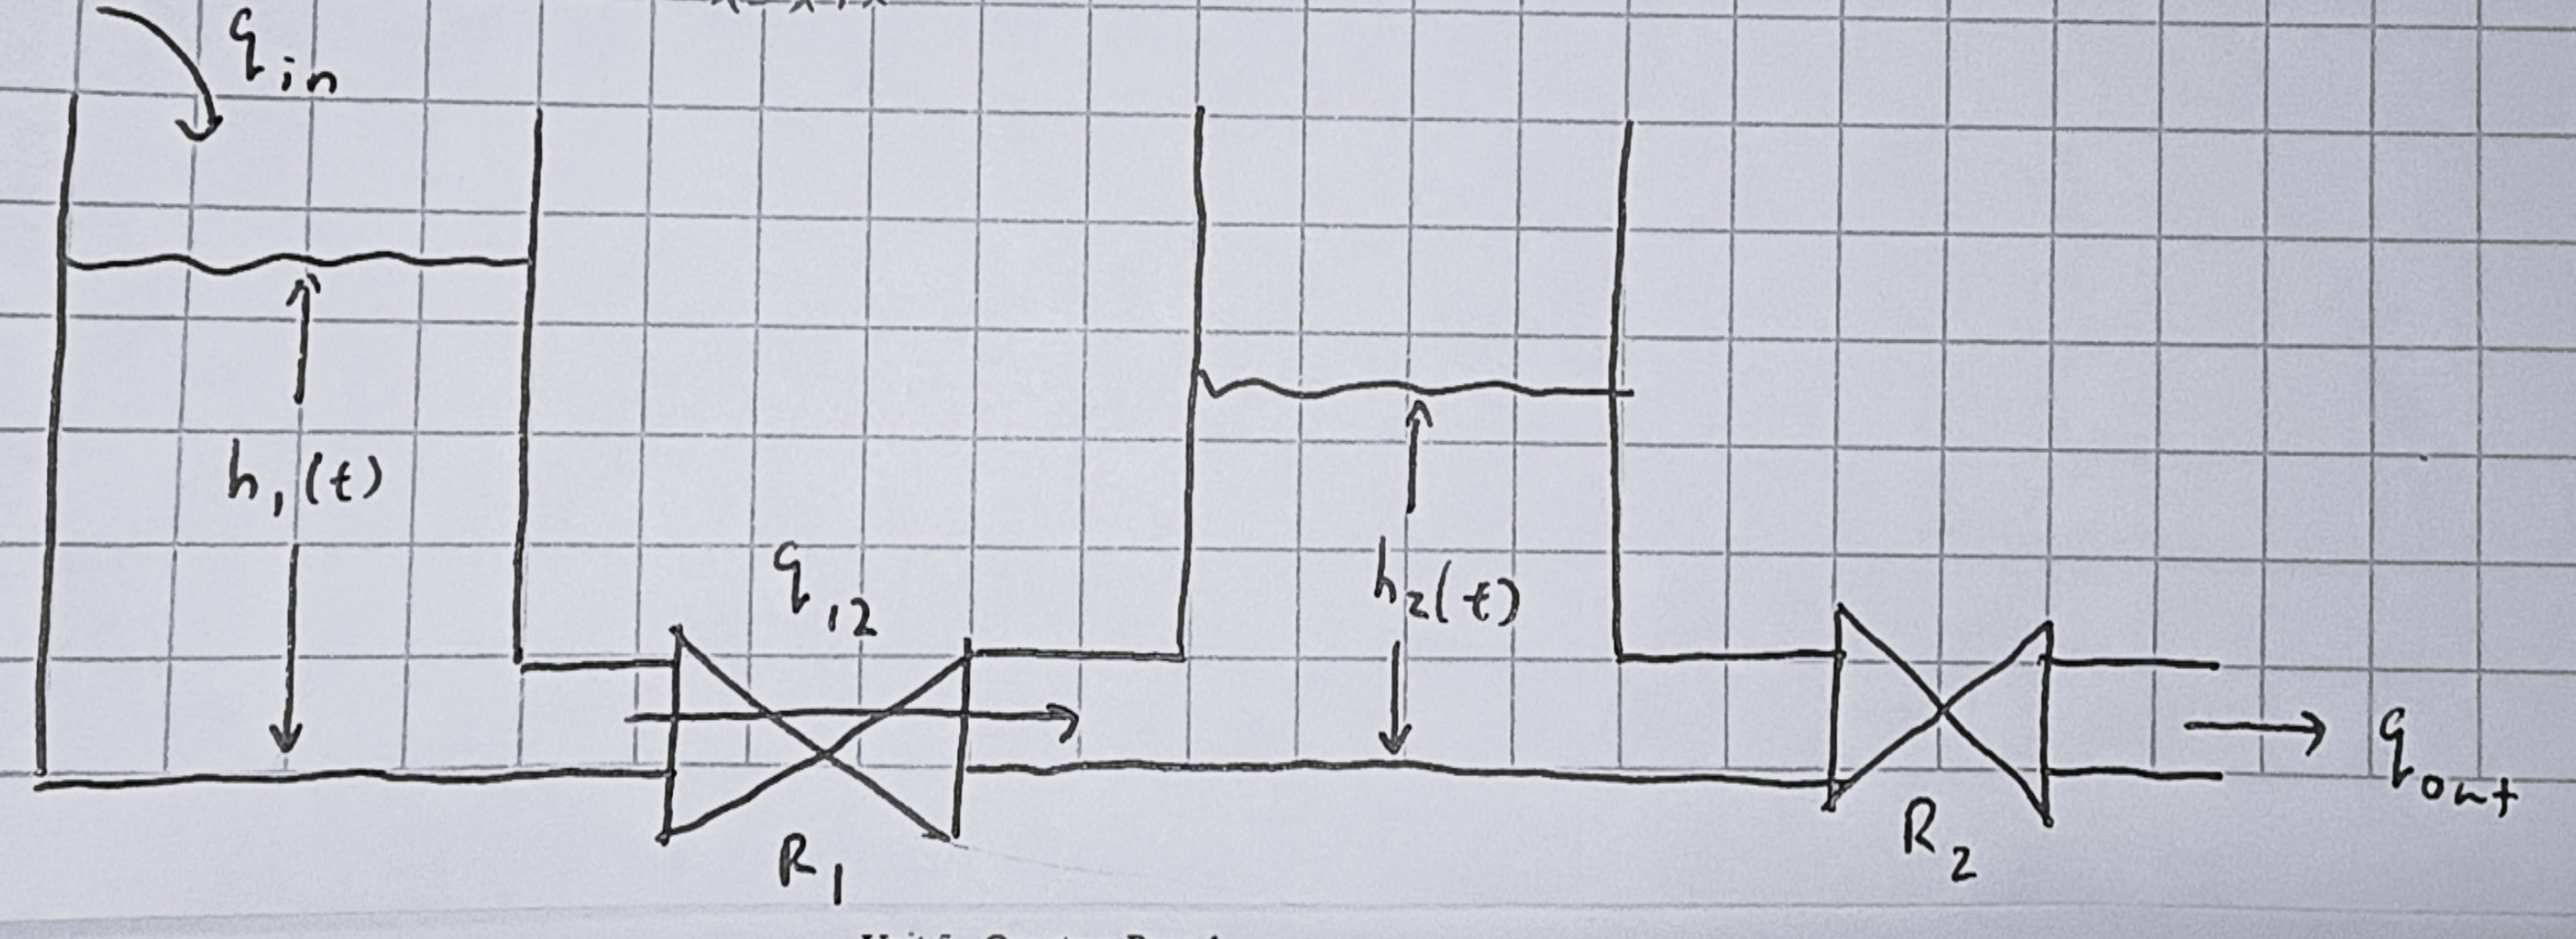
\includegraphics[width=0.65\textwidth]{Fluid R_h.jpg}
\end{center}
\[q_{12} = \frac{h_{12}}{R_1},\quad q_{\text{out}} = \frac{h_2}{R_2}\]
\section*{Fluid Capacitance}
Fluid capacitance ($C$) defines how much fluid we need to add to get a change in pressure. A high capacitance means that we need to add a lot of fluid to get a small change in pressure, while a low capacitance means that we only need to add a little bit of fluid to get a large change in pressure. Note that pressure changes is due to \textbf{hydrostatic pressure} ($p=\rho g h$), so the change in pressure is proportional to the change in fluid level. \\\\
Similar to resistance, we have two definitions for fluid capacitance depending on whether we are modeling pressure difference or head difference. However, it is important to note that we can convert between pressure and head using the hydrostatic pressure relationship, so these two definitions describe the \textit{same physical phenomenon} but we use it purely for convenience depending on the problem.\\\\
\textbf{Head}\\
Consider the following tank with cross-sectional area $A$ and head $h$:
\begin{center}
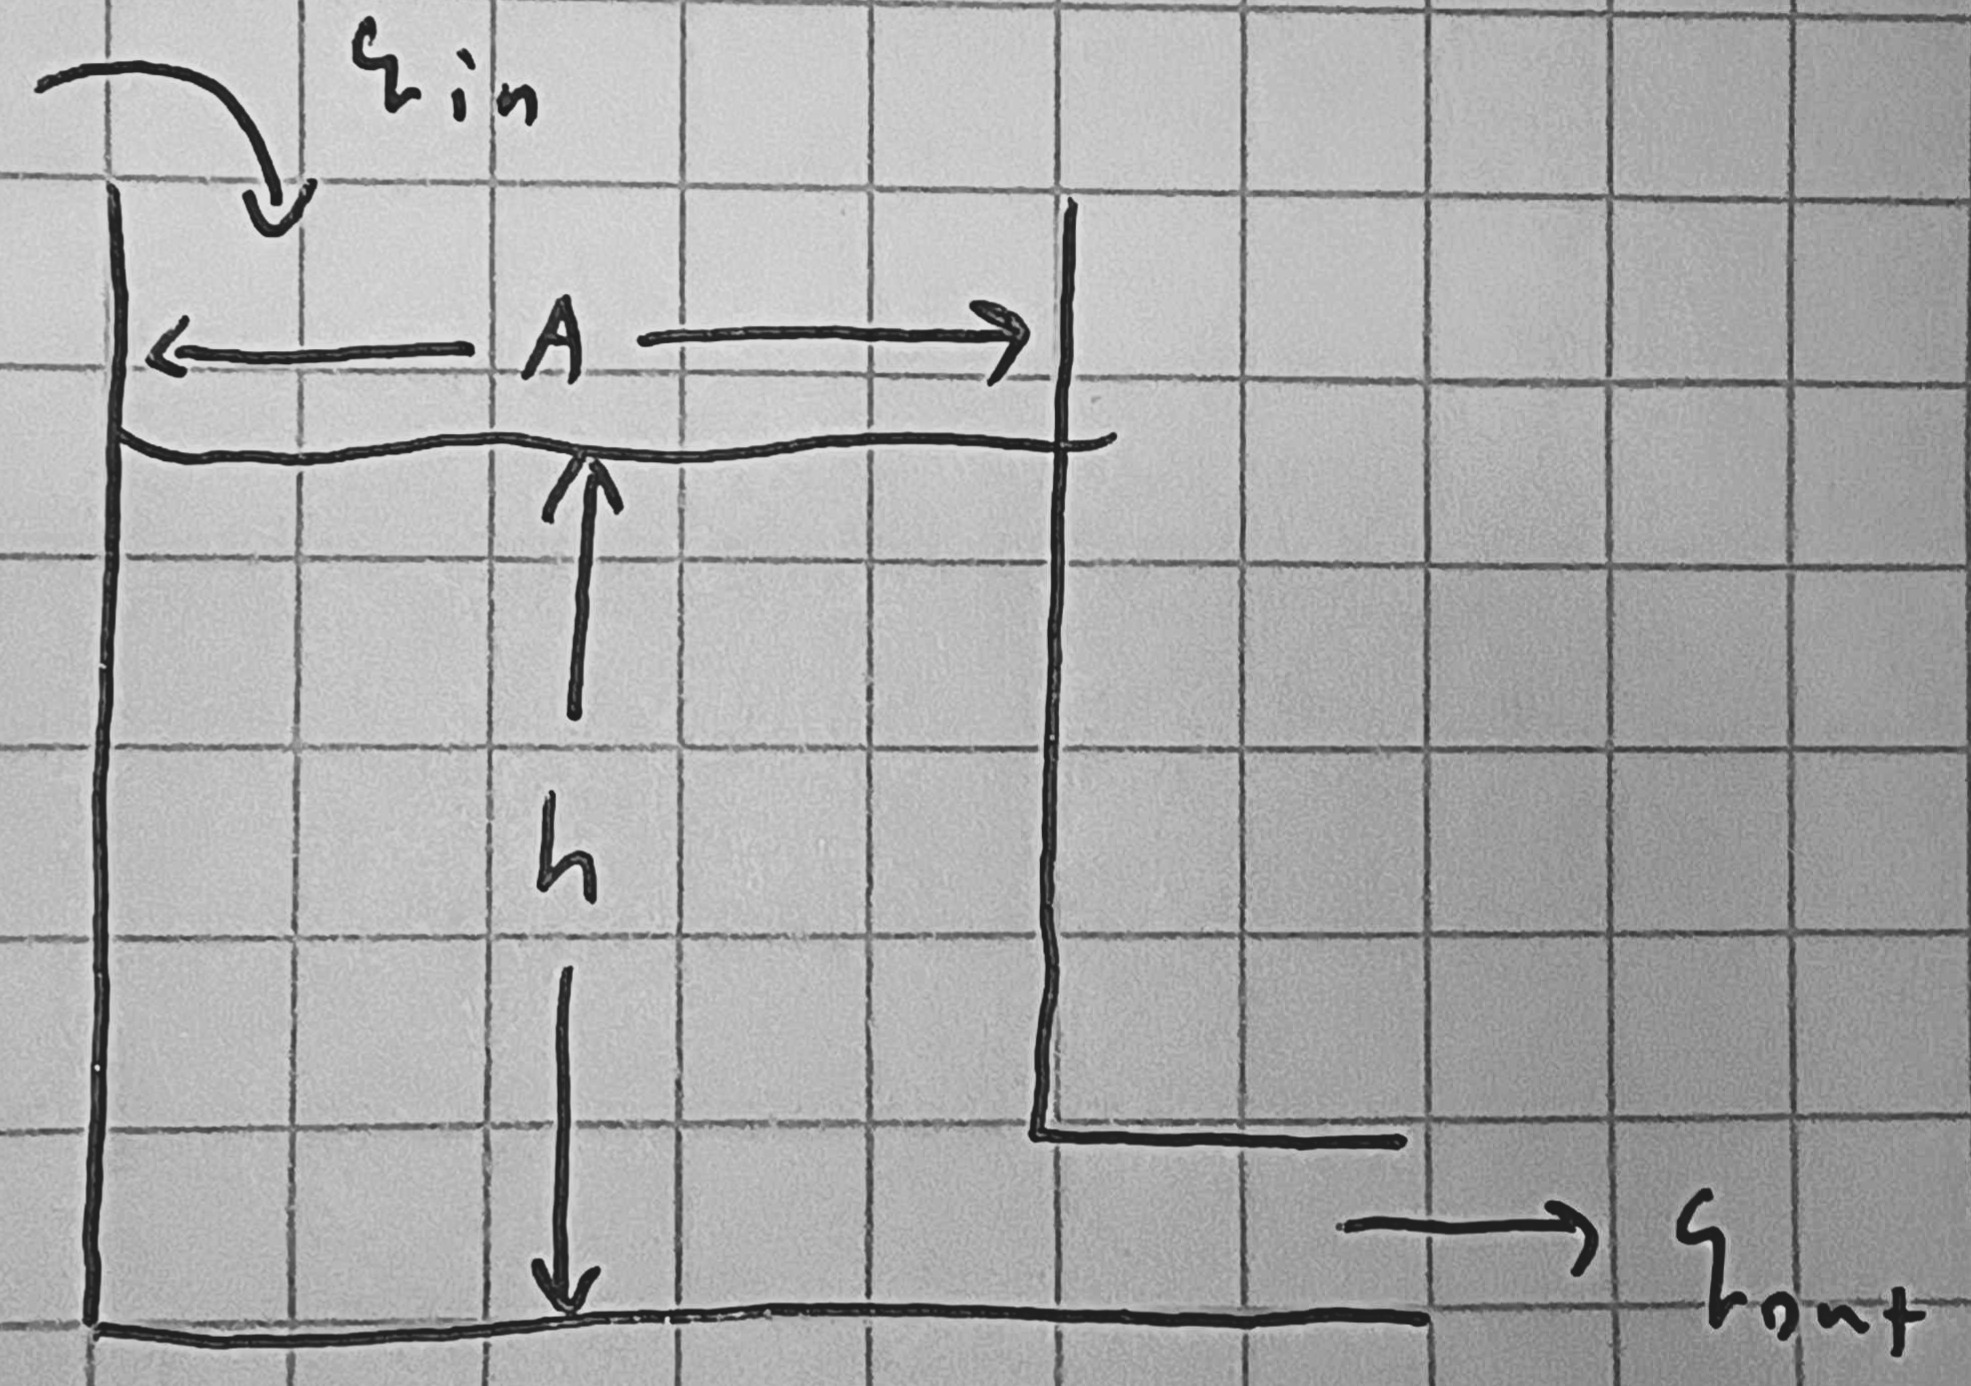
\includegraphics[width=0.35\textwidth]{Fluid C.jpg}
\end{center}
We begin with the conservation of mass:
\[\frac{dm}{dt} = \sum \dot{m}_{\text{in}} - \sum \dot{m}_{\text{out}}\]
Since $m=\rho \vol \implies \dot{m} = \rho \dot{\vol}$ and $\dot{\vol} = q$ ($\vol$ is the fluid volume), we can rewrite the conservation of mass for a single inlet, single outlet system as:
\[\frac{d(\rho \vol)}{dt}=\rho q_\text{in}-\rho q_\text{out}\]
Assuming the fluid is incompressible (constant density), we get:
\[\boxed{\frac{d\vol}{dt} = q_\text{in} - q_\text{out}}\]
From geometry, we know that $\vol=Ah$, thus we have the head capacitance relationship:
\[\boxed{A\frac{dh}{dt} = q_\text{in} - q_\text{out},\quad C_h = A\quad\text{[m$^2$]}}\]
\textbf{Pressure}\\
For the pressure definition of fluid capacitance, we can use the hydrostatic pressure relationship to convert from head to pressure:
\[A\frac{dh}{dt} = q_\text{in} - q_\text{out}, \quad p = \rho g h\]
\[\implies A \frac{d(\frac{p}{\rho g})}{dt} = q_\text{in} - q_\text{out}\]
\[\implies \boxed{\frac{A}{\rho g}\frac{dp}{dt} = q_\text{in} - q_\text{out},\quad C_p = \frac{A}{\rho g}\quad\left[\frac{\mathrm{m}^4\,\mathrm{s}^2}{\mathrm{kg}}=\frac{\mathrm{m}^5}{\mathrm{N}}\right]}\]
\textbf{General Definition}\\
Generally, we define the following relationship for fluid capacitance:
\[\boxed{\vol=Cp_{12}\implies C=\frac{d\vol}{dp}}\]
Thus, fluid capacitance is analogous to the definition of electrical capacitance $Q=CV$ where $Q$ is the stored charge and $V$ is the voltage across the capacitor. Additionally, differentiating both sides with respect to time gives us the relationship between flow rate and pressure difference:
\[q = C\frac{dp}{dt}\]
This is also analogous to the relationship between current and voltage for an electrical capacitor $i=C\frac{dv}{dt}$.
\section*{Fluid Inertance}
Fluid inertance ($I$) defines how hard it is to change the fluid flow rate, since it requires pressure to overcome the \textit{momentum} or inertia of the fluid. While we can neglect this effect by assuming steady-state flow ($\frac{dq}{dt}=0$), we still make note of it.\\\\
Consider the following pipe with length $L$ and cross-sectional area $A$. Starting with Newton's second law:
\[\sum F=m\frac{dv}{dt}\]
The net applied force on the fluid is due to the pressure difference across the pipe:
\[\sum F = p_1A - p_2A = p_{12}A\]
The mass of the fluid in the pipe is given by $m=\rho \vol = \rho AL$, and the velocity of the fluid is given by $q=Av$, thus we can rewrite Newton's second law as:
\[p_{12}A = \rho AL \frac{dv}{dt}\]
\[\implies p_{12}A = \rho AL \frac{d(\frac{q}{A})}{dt}\]
Thus, we have the relationship for fluid inertance:
\[\boxed{p_{12} = \frac{\rho L}{A}\frac{dq}{dt},\quad I = \frac{\rho L}{A}\quad\left[\frac{\text{N}\cdot\text{s}^2}{\text{m}^5}\right]}\]
Or by using the hydrostatic pressure relationship, we can convert from pressure difference to head difference:
\[\boxed{h_{12} = \frac{L}{Ag}\frac{dq}{dt},\quad I = \frac{L}{Ag}\quad\left[\frac{\text{m}}{\text{m}^2(\text{m/s}^2)}=\frac{\text{s}^2}{\text{m}^2}\right]}\]
Note that this is analogous to the relationship between voltage and current for an electrical inductor $V=L\frac{di}{dt}$.
\section*{Governing Equations}
To derive the governing equations for a fluid system, we can use the conservation of mass and energy principles.\\\\
\textbf{Conservation of Mass}\\
At any point where pipes meet, or a tank exists, we know that by the conservation of mass:
\[\frac{d\vol}{dt} =  q_{\text{in}} -  q_{\text{out}}\]
Where $\vol$ is the fluid volume in the tank. In the case of a pipe junction, there is \textit{no storage of fluid}, thus $d\vol/dt=0$.\\\\
We can then replace $q_{\text{in}} -  q_{\text{out}}$ with the relationships for capacitance and resistance (and inertance if needed) to get the governing equations for the system.
\section*{Analogous Systems}
\begin{center}
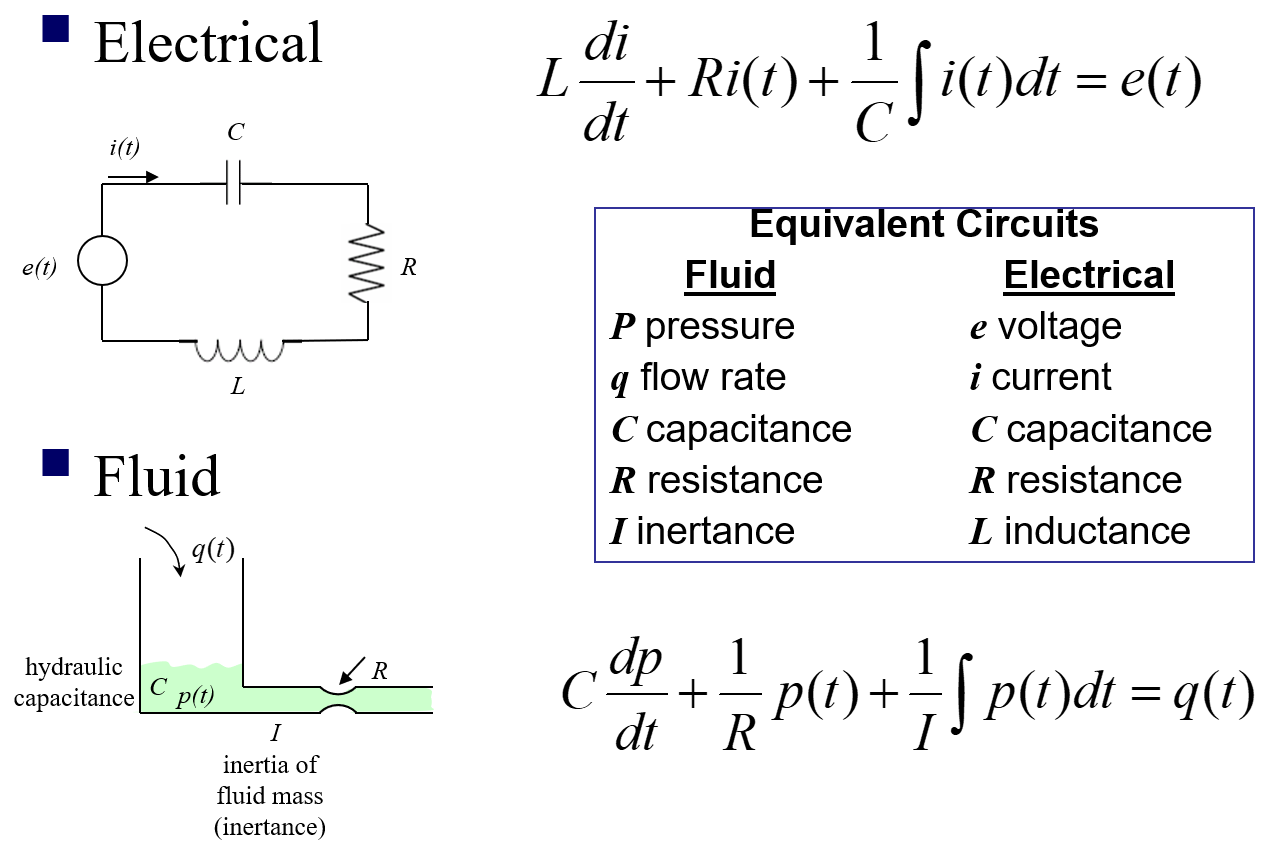
\includegraphics[width=0.8\textwidth]{Fluid sys.png}
\end{center}
\noindent\hrule
\vspace{1em}
\newpage
\begin{center}
{\LARGE Thermal Systems\par}
\end{center}
Now that we have built and understanding of modeling resistance and capacitance in fluid systems, the same modeling techniques can be applied to thermal systems.
\begin{table}[h]
\centering
\renewcommand{\arraystretch}{1.5}
\begin{tabular}{|l|l|l|}
\hline
 & \textbf{Fluid System} & \textbf{Thermal System} \\ \hline
\textbf{Effort (Potential)} & Pressure ($p$) or Head ($h$) & Temperature ($T$) \\ \hline
\textbf{Flow (Rate)} & Volumetric Flow ($q$) & Heat Flow Rate ($q$) \\ \hline
\textbf{Storage (Capacitance)} & Tank Area ($A$) & Thermal Mass ($mc_p$) \\ \hline
\textbf{Opposition (Resistance)} & Pipe Friction ($R$) & Insulation ($R$) \\ \hline
\end{tabular}
\end{table}

\end{document}
